\chapter{State of the Art}
\label{chap:sota}

\begin{tcolorbox}[colback=royallavender!40]
The content of this Chapter has already been partially included in the articles published during this Thesis~\citep{esteves_odrl_2021,esteves_analysis_2022,asgarinia_who_2023,esteves_using_2023,florea_is_2023}.
\end{tcolorbox}

This Chapter presents the state of the art on the representation of policies and personal data processing metadata in the context of determining access to decentralised personal data systems, focusing on solutions that use Semantic Web technologies and cater to data protection law requirements.
Since there are different areas being covered in this state of the art analysis, each topic will be first introduced with a list of criteria used to perform said analysis.
The prefixes and namespaces used in the Listings in this Chapter are explicitly defined in the \hyperref[sec:namespaces]{Namespaces list}.

Thus, a literature review was performed in the subsequent areas, following the methodology described in Section~\ref{sec:technical_review}:

\begin{itemize}
    \item [\textbf{\ref{sec:sota_solid}}] Decentralising the access to personal data with Solid
    \item [\textbf{\ref{sec:sota_vocabularies}}] Representing personal data processing information
    \item [\textbf{\ref{sec:sota_policies}}] Using policy languages to specify access control conditions
\end{itemize}

Through this analysis, a series of gaps and challenges in the representation of privacy terms was identified, in order to have a legally-aligned Solid environment, and is described in Section~\ref{sec:challenges}.

\section{Decentralising the access to personal data with Solid}
\label{sec:sota_solid}

As attested in Section~\ref{sec:def_decentralised_env}, current efforts are underway to decentralise today's Web. By decoupling data from applications, Web users will have their data stored in an environment they can control and can choose what data they want to make publicly accessible or accessible only to certain users while using their application of choice to manage said data.
This represents a significant paradigm shift regarding users' current online experience -- instead of being locked away in Big Tech companies' storage servers, data can be stored on individual personal datastores maintained by a provider chosen by the user or hosted by the user itself on its private server.
In this context, the Solid project~\citep{sambra_solid_2016,mansour_demonstration_2016} has been gaining prominence as it relies on Web standards to achieve this degree of decentralisation -- its ultimate goal is to give Web users a personal datastore, i.e., a Pod, per user, with a granular access control system managed by the user, which they can use to select which people and/or applications have access to the resources stored on their Pod.
As such, with Solid, applications and the companies behind them do not store the (personal) data of their users, acting only as interfaces that can read, write, or append data to/from Pods.
Such an ecosystem \textit{``fosters innovation and competition through separate markets for data and applications''}~\citep{verborgh_paradigm_2017}, while allowing Web users to exert a degree of control over their data that is currently impossible to wield.

In particular, the Solid protocol~\citep{capadisli_solid_2022} describes how servers and apps should behave by relying on the following Web standards:

\begin{itemize}
    \item HTTP~\citep{fielding_http_2022} -- The Hypertext Transfer Protocol describes an architecture and semantics for \textit{``distributed, collaborative, hypertext information systems''} to share data.
    \item RDF~\citep{cyganiak_rdf_2014} -- The Resource Description Framework defines a data model to represent information in the Web, including a schema~\citep{brickley_rdf_2014} and serialisation syntaxes for storing and exchanging RDF such as Turtle~\citep{prudhommeaux_rdf_2014} and JSON-LD~\citep{gregg_kellogg_json-ld_2020}.
    \item LDP~\citep{speicher_linked_2015} -- The Linked Data Platform specification expresses how to use \textit{``HTTP for accessing, updating, creating and deleting resources from servers that expose their resources as Linked Data''}.
    \item SPARQL~\citep{harris_sparql_2013} -- The SPARQL language can be used to query RDF databases. %Solid also uses a subset of SPARQL UPDATE through HTTP PATCH queries.
    \item WebID-TLS~\citep{story_webid-tls_2014} -- A protocol that uses WebIDs to authenticate users on the Web.
    \item OIDC~\citep{sakimura_openid_2014} -- The OpenID Connect standard is an authentication protocol to assert the user's identity. 
\end{itemize}

Moreover, Table \ref{tab:definitions} provides an overview of Solid-related concepts, their definitions, and corresponding classes and properties already modelled in Solid-related vocabularies.
The authentication and authorisation protocols compose Solid's two main building blocks -- an up-to-date list of Solid specifications, including technical reports for both aforementioned building blocks, is maintained by the Solid Community Group at \url{https://solidproject.org/TR/}.
Authentication is a necessary feature to identify users when they want to log into their Pod and/or when they want to use an app to perform a certain action over resources stored in their Pod.
Thus, Solid's authentication protocol uses Solid's WebID specification to identify agents through URIs, as specified in Table~\ref{tab:definitions}, which when dereferenced return a WebID profile document that should include information regarding the identity provider chosen by the Solid user and the Pod storage location and may include information regarding an available inbox where users and applications can leave messages to the user~\citep{balseiro_solid_2022}.
In addition, to verify the identity of agents, the Solid Protocol recommends the usage of the Solid OIDC protocol\footnote{A Solid-OIDC Primer~\citep{morgan_oidcprimer_2022} is also being developed to provide additional knowledge on Solid OIDC's authentication flows.}~\citep{coburn_oidc_2022}, however additional authentication methods, such as the previously mentioned WebID-TLS, can also be implemented.

The authorisation protocol specifies mechanisms used by Solid servers to reply to requests of particular users or apps to have access to certain resources, containers of resources, or even to the whole Pod.
Furthermore, the Solid protocol states that a Solid server \textit{``MUST conform to either or both Web Access Control (WAC) and Access Control Policy (ACP) specifications''} in order for it to be a compliant Solid server.
Specific authorisation use cases and requirements are documented by the~\cite{solid_editorial_team_use_2023} and further details on the authorisation methods will be given in Section~\ref{sec:sota_solid_access_control}.
In addition to the authorisation specifications, there is a third protocol being developed to ensure data interoperability and (re)usability across Pod providers, agents, and applications -- the Solid Application Interoperability (SAI) specification~\citep{bingham_interop_2023}.

\begin{landscape}
\begin{table}[p]
\caption[Overview of Solid-related concepts.]{Overview of Solid-related concepts, their definitions, and related terms modelled on Solid specifications.}
\label{tab:definitions}
\begin{tabular}{c||l|c}
\textbf{Concept} & \textbf{Definition} & \textbf{Solid vocabularies} \\ \hline\hline
Pod & A personal datastore that conforms to the Solid protocol & \texttt{pim:Storage} \\ \hline
Resource & \begin{tabular}[c]{@{}l@{}}Target asset stored in a Pod identified by a URI. Container resources can\\ contain other resources including containers\end{tabular} & \begin{tabular}[c]{@{}c@{}}\texttt{acl:accessTo}, \\ \texttt{acp:target} \end{tabular} \\ \hline
Inbox & Container resource for messages sent to an agent & \begin{tabular}[c]{@{}c@{}}\texttt{ldp:inbox}, \\ \texttt{interop:hasInbox}\end{tabular} \\ \hline
Server & Server capable of hosting resources and responding to resource requests & \\ \hline
App & An application that reads and writes data to Pods & \begin{tabular}[c]{@{}c@{}}\texttt{interop:Application}, \\ \texttt{acp:client}, \texttt{acl:origin}\end{tabular} \\ \hline
Agent & A person, social or virtual entity identified by a URI & \begin{tabular}[c]{@{}c@{}}\texttt{interop:Agent}, \\\texttt{acl:agent}, \texttt{acp:agent}\end{tabular} \\ \hline
\begin{tabular}[c]{@{}c@{}}Pod \\ Owner\end{tabular} & \begin{tabular}[c]{@{}c@{}}Agent that has control over all resources in a Pod including access control\\ resources\end{tabular} & \begin{tabular}[c]{@{}c@{}}\texttt{solid:owner}, \\ \texttt{acp:owner}\end{tabular} \\ \hline
WebID & \begin{tabular}[c]{@{}l@{}}URI that acts as a primary identifier for agents, which, when dereferenced,\\ resolves to an identity profile document (WebID profile)\end{tabular} & \\ \hline
\begin{tabular}[c]{@{}c@{}}Identity \\ Provider\end{tabular} & Entity implementing the identity service capable of authenticating a WebID & \begin{tabular}[c]{@{}c@{}}\texttt{solid:oidcIssuer}, \\ \texttt{acp:issuer}\end{tabular} \\ \hline
\begin{tabular}[c]{@{}c@{}}Pod \\ Provider\end{tabular} & Entity providing the storage space and maintaining the server implementation & \\ \hline
Policy & Conditions for accessing the Pod and its resources & \texttt{acp:Policy} \\ \hline
Registry & \begin{tabular}[c]{@{}c@{}}Records where agents can store and find different types of data for different\\ purposes\end{tabular} & \texttt{interop:Registry}
\end{tabular}
\end{table}
\end{landscape}

\subsection{Access control and interoperability in Solid}
\label{sec:sota_solid_access_control}

As discussed in the previous Section, there are two distinct access control methods being specified in the Solid ecosystem -- both use URIs to identify resources and users, while WAC~\citep{capadisli_wac_2022} relies on ACLs and ACP~\citep{bosquet_acp_2022} on Access Control Resources (ACRs) to specify who is authorised or refused access and access grants to represent the final authorisation decision.
While server providers can implement only one of the authorisation protocols, Solid applications can not do the same or else they will not work with server providers that use a distinct protocol from the one they choose to implement.
Listings~\ref{list:wac} and~\ref{list:acp} provide examples of both types of access control statements.
As is visible by the examples, both solutions do not have the depth to deal with the users \textit{`Right to be Informed'} \hyperref[art:13-14]{(Arts. 13 and 14)}~\citeyearpar{noauthor_regulation_2016}, since these models do not contain the terms to specify the purpose for accessing data on Pods, the personal data categories being consulted, used legal basis or even information on the identity of application developers.

\begin{listing}[ht]
\caption[WAC authorisation.]{WAC authorisation that makes a WebID profile, \url{https://solidweb.me/besteves4/profile/card}, readable by any agent.}
\label{list:wac}
\begin{minted}{turtle}
<#public> a acl:Authorization ;
    acl:agentClass foaf:Agent ;
    acl:accessTo <https://solidweb.me/besteves4/profile/card> ;
    acl:mode acl:Read .
\end{minted}
\end{listing}

\begin{listing}[ht]
\caption[ACP authorisation.]{ACP authorisation that makes a WebID profile, \url{https://solidweb.me/besteves4/profile/card}, issued by \url{https://solidweb.me/}, readable by any agent using any application.}
\label{list:acp}
\begin{minted}{turtle}
<#public> a acp:AccessGrant ;
    acp:grant acl:Read ;
    acp:context [
        acp:agent acp:PublicAgent ;
        acp:target <https://solidweb.me/besteves4/profile/card> ;
        acp:client acp:PublicClient ;
        acp:issuer <https://solidweb.me/> ] .
\end{minted}
\end{listing}

Moreover, these access protocols were deemed not enough to ensure the interoperability of agents, data, and applications, and as such an interoperability specification is being developed to describe the implementation of agent, data, and access registries, to track user interactions with other agents, to keep records of where data is being stored and to manage access grants given to other agents~\citep{bingham_interop_2023}.
Listing~\ref{list:interop_registryset} provides an example of a registry set that should only be readable by the Pod owner and Listing~\ref{list:interop_authz_registry} an example of an authorisation registry, which contains an \texttt{AccessAuthorization} for the \texttt{projectron} app which requires data with a particular shape\footnote{SAI assumes the use of ACL access modes which are still not approved, e.g., \texttt{acl:Create}, \texttt{acl:Update}, \texttt{acl:Delete}, and are under discussion on the Solid CG authorisation panel (see the issue at \url{https://github.com/solid/authorization-panel/issues/253}).}.
While SAI is a step forward in Solid towards having a more transparent ecosystem, it is still in the early stages of development, and as such it is still not clear how this specification will fit in with the existing access control protocols or how it is going to be implemented/enforced.
In addition, as is illustrated by Listing~\ref{list:interop_authz_registry}, SAI does not entirely fulfil GDPR requirements, e.g., it does not provide transparency regarding the purpose for access or which type of data is being accessed nor does it provide information regarding the identity of the entities that develop/provide the apps.

\begin{listing}[ht]
\caption[SAI registry set.]{Registry set, established according to the SAI specification, that stores private information regarding the storage location of registries of \url{https://solidweb.me/besteves4/}.}
\label{list:interop_registryset}
\begin{minted}{turtle}
PREFIX beatriz-registry: <https://solidweb.me/besteves4/registry/>
PREFIX beatrizWork-registry: <https://solidweb.me/besteves4-work/registry/>

beatriz-registry: a interop:RegistrySet ;
  interop:hasAgentRegistry beatriz-registry:agents ;
  interop:hasAuthorizationRegistry beatriz-registry:authz ;
  interop:hasDataRegistry beatriz-registry:data , beatrizWork-registry:data .
\end{minted}
\end{listing}

\begin{listing}[htp]
\caption[SAI authorisation registry.]{Authorisation registry of \url{https://solidweb.me/besteves4/}.}
\label{list:interop_authz_registry}
\begin{minted}{turtle}
PREFIX beatriz-authz: <https://solidweb.me/besteves4/registry/authz/>
PREFIX projectron: <https://projectron.app/>
PREFIX projectron-shapetrees: <https://projectron.app/shapetrees/>

beatriz-registry:authz a interop:AuthorizationRegistry;
    interop:hasAccessAuthorization beatriz-authz:projectron .

beatriz-authz:projectron a interop:AccessAuthorization ;
    interop:grantedBy <https://solidweb.me/besteves4/profile/card#me> ;
    interop:grantedWith <https://authz.agent/id> ;
    interop:grantedAt "2023-07-31T11:53:01Z"^^xsd:dateTime ;
    interop:grantee projectron:id ;
    interop:hasAccessNeedGroup projectron:need-group ;
    interop:hasDataAuthorization beatriz-authz:54a1b6a0 .

projectron:need-group a interop:AccessNeedGroup ;
    interop:accessNecessity interop:accessRequired ;
    interop:accessScenario interop:PersonalAccess ;
    interop:authenticatesAs interop:SocialAgent ;
    interop:hasAccessDescriptionSet projectron:access-en ;
    interop:hasAccessNeed projectron:need-project .

projectron:need-project a interop:AccessNeed ;
    interop:registeredShapeTree projectron-shapetrees:ProjectTree ;
    interop:accessNecessity interop:accessRequired ;
    interop:accessMode acl:Read, acl:Create ;
    interop:creatorAccessMode acl:Update, acl:Delete .

beatriz-authz:54a1b6a0 a interop:DataAuthorization ;
    interop:grantee projectron:id ;
    interop:registeredShapeTree projectron-shapetrees:ProjectTree ;
    interop:accessMode acl:Read, acl:Create ;
    interop:creatorAccessMode acl:Update, acl:Delete ;
    interop:scopeOfAuthorization interop:All ;
    interop:satisfiesAccessNeed projectron:need-project .
\end{minted}
\end{listing}

Furthermore, the idea of having registries of data and applications is also compatible with the graph-centric interpretation of a Pod debated by~\cite{dedecker_whats_2022}.
Certain apps might require the presence of particular data stored in a particular container -- this will cause an interoperability problem as it is something that cannot be standardised across the ecosystem for all apps.
With a graph-centric approach, \textit{``each Solid pod is a hybrid, contextualized knowledge graph, wherein `hybrid' indicates first-class support for both documents and RDF statements, and `contextualized' the ability to associate each of its individual documents and statements with metadata such as policies, provenance, and trust''}.
With such metadata, including context and provenance metadata, distinct views of the Pod can be rendered as required by different applications or agents.
Moreover, data request policies can simply be appended to the \textit{`Pod as a Graph'}, without the need to have it hard-coded in the app, and can be viewed by users using graphic-centric Solid apps.

\subsection{Solid and data protection}
\label{sec:sota_solid_data_protection}

Only recently has the debate on data protection reached the concerns of Solid's developers, mainly with regard to issues of control and privacy of personal data.
In addition, beyond the access control mechanisms discussed in the previous Section, there are also researchers starting to work on \textit{`usage control'}, a process which has as its main concern the enforcement of the users' policies after the access to the data has already been given~\citep{akaichi_semantic_2022,havur_greater_2020}.
As such, in this Section, we describe the existing body of work on data protection and governance aspects of Solid-related technologies, with a particular focus on GDPR-related academic and industrial research.

\paragraph{Exercising of data subject rights} 
\cite{de_mulder_prov4itdata_2021} developed PROV4ITDaTa\footnote{The source code is available at \url{https://github.com/RMLio/prov4itdata-web-app}, under an MIT license (accessed on 14 August 2023).}, a configurable application that facilitates the exercising of the data subject's \textit{`right to data portability'}~\hyperref[art:20]{(Art. 20)}~\citeyearpar{noauthor_regulation_2016}, using open sources resources such as RML.io\footnote{\url{https://rml.io/} (accessed on 14 August 2023)}~\citep{dimou_rml_2014} -- to access and generate interoperable Linked Data datasets using the Schema.org or DCAT vocabularies, Solid -- to store the datasets, and Comunica\footnote{\url{https://comunica.dev/} (accessed on 14 August 2023)}~\citep{taelman_comunica_2018} -- to query the datasets, and promotes transparency by automatically generating and recording provenance metadata using the PROV Ontology standard.
The PDS Interop collaboration~\citeyearpar{noauthor_pds_2021}, an effort that started with the goal to make Solid and Nextcloud\footnote{\url{https://nextcloud.com/} (accessed on 20 August 2023)} interoperable, also developed an app, the Solid Migrator App\footnote{The source code is available at \url{https://github.com/pdsinterop/solid-migrator-app}, under an MIT license (accessed on 20 August 2023).}, to assist in the migration of Pod resources to a different Pod, independently of the Pod provider.

\paragraph{GDPR principles}
\cite{pandit_making_2023} describes Solid as a \textit{`cloud technology'}, according to ISO standards, provides a theoretical discussion on how GDPR principles apply to Solid and suggests how to extend its specifications to deal with such requirements.
\cite{esposito_assessing_2023} also provide a theoretical analysis of technical security and privacy measures to assist Solid developers in complying with the GDPR -- a mapping of Solid actors and respective legal roles is provided for accountability, as well as security measures to ensure data confidentiality and minimisation and protocols to safeguard the data subjects' rights to be notified~\hyperref[art:19]{(Art. 19)}~\citeyearpar{noauthor_regulation_2016}, to object~\hyperref[art:21]{(Art. 21)}~\citeyearpar{noauthor_regulation_2016} and to not be a target of automated decision-making~\hyperref[art:22]{(Art. 22)}~\citeyearpar{noauthor_regulation_2016}.
\cite{van_damme_towards_2022} present a qualitative analysis of a series of plenary sessions with academia, governments, citizens, and industry regarding the adoption of decentralised personal datastore technologies. The main challenges that were identified are related to social, technical, legal, and ecosystem issues, which need to be considered for the \textit{``development of an interdisciplinary research agenda''}. In terms of legal challenges, the core aspects that were discussed are related to control, portability, compliance, accountability, delegation of consent, and the usage of other legal bases such as legitimate interests. The role of intermediates, promoted by the DGA, was also discussed. % Use cases related to mobility, media, health, finance and administration were also discussed.
Digita\footnote{\url{https://www.digita.ai/} (accessed on 15 August 2023)}, a Belgian startup that offers Solid-based identity and storage solutions, published a research report reflecting on accountability aspects related to the implementation of Solid products, mainly regarding the lawfulness of data usage and transfer to recipients, particularly based on consent, and the specificity and compatibility of purposes~\citep{de_bot_data_2021}.
\cite{bailly_prototyping_2023} propose to use the SAI and DPV vocabularies to specify access and usage control policies, respectively, and provide a prototype User Interface (UI) for users to consent to data requests\footnote{The source code is available at \url{https://github.com/HBailly/solid-auth-ui/}, under a GNU General Public License v3.0 (accessed on 15 August 2023).}, which the authors found to have a low score in terms of usability.
% athumi (flemish data utility company) not discussed, find paper?

\paragraph{Domain-specific use cases}
Several health-related use cases have been developed by the Solid research community.
Among them, TIDAL\footnote{The source code is available at \url{https://github.com/sunchang0124/TIDAL}, under an MIT license (accessed on 15 August 2023).} (ciTIzen-centric DAta pLatform), a Solid-powered application, has been developed by~\cite{sun_citizen-centric_2023} for healthcare researchers to request consent from citizens to use their data for health-related research. DPV is used to limit the purpose for which the data can be used, DPV-PD and other health-related vocabularies to restrict the categories of personal data, and privacy-preserving data analysis algorithms to preserve data confidentiality.
Janeiro Digital\footnote{\url{https://www.janeirodigital.com/} (accessed on 15 August 2023)}~\citeyearpar{noauthor_janeiro_nodate} is working with the United Kingdom's National Health Service (NHS) to manage and use patient data from several systems, providing patients with individual Solid Pods and giving healthcare professionals access to data through the Solid protocol.
\cite{ammar_personal_2020,ammar_using_2021} discuss the implementation of a \textit{`Personal Health Library'} using Solid \textit{``to deliver tailored push notifications to support behavior change related to chronic disease self-care''} based on sensor readings and other information.
In addition, they are developing an app to allow users to decide what data should be stored in the Pod, and who should have access to it, and to share their data with other research initiatives.

In addition to the work of~\cite{de_bot_data_2021}, \cite{chugunov_streamlining_2020} also focus on government-related use cases. In this work, a Solid app for Flemish citizens, that allows them to share data with government administrations and to reuse said data in different contexts, is described to increase the accuracy of personal data which is difficult to keep updated, e.g., telephone numbers or email addresses, and to allow data portability.
\citeauthor{wang_enhancing_2020}'s thesis also discusses the usage of Solid to enhance governmental services, including provisions to improve the access~\hyperref[art:15]{(Art. 15)}~\citeyearpar{noauthor_regulation_2016} and rectification~\hyperref[art:16]{(Art. 16)}~\citeyearpar{noauthor_regulation_2016} rights exercised in this context, including a use case scenario of applying to a social house and dealing with the subsequent changes to the address. 

Karamel\footnote{\url{https://karamel.career/} (accessed on 20 August 2023)} also partnered with Digita to create a human resources platform for applicants and recruiters to find new jobs~\citep{verstraete_solid_2022} -- users can manage data stored in Solid Pods through an app that allows applicants to revoke access and to request to be forgotten~\hyperref[art:17]{(Art. 17)}~\citeyearpar{noauthor_regulation_2016} by recruiters.

\cite{toth_preserving_2022} developed a prototype architecture for the domain of hospitality where users can use Solid applications to book/manage accommodations and edit personal information. This proof of concept\footnote{The source code is available at \url{https://github.com/gergelyth/solid-hotel}, under an MIT license (accessed on 21 August 2023).} allows its users to request deletion~\hyperref[art:17]{(Art. 17)}~\citeyearpar{noauthor_regulation_2016} and rectification~\hyperref[art:16]{(Art. 16)}~\citeyearpar{noauthor_regulation_2016} of data and of copies of said data.

\cite{van_de_wynckel_solidbased_2022} are researching the usage of Solid to develop transparent indoor positioning systems that store individual and sensor data in Solid Pods in an interoperable format. In addition, they developed an app that reads the user’s personal position, orientation, and velocity from the Pod and displays them along with additional information\footnote{The source code is available at \url{https://github.com/OpenHPS/ipin2022-solid/} (accessed on 23 August 2023).}.

The described solutions can be compared through Figure~\ref{fig:solid_sota}.
Each solution was analysed in terms of whether it assists in the exercising of data subject rights or the implementation of a certain GDPR principle, as well as the type of solution developed by the authors of the paper.
Works describing Solid apps are marked with a \textbf{black} shape, identity provider solutions with a \textbf{\textcolor{orange}{orange}} shape, Pod provider solutions with a \textbf{\textcolor{blue}{blue}} shape and theoretical work with a \textbf{\textcolor{red}{red}} shape.
In addition, works marked with a $\medcircle$ discuss a government-related use case, $\medtriangleup$ a health-related use case, $\meddiamond$ a hospitality-related use case, \faStarO\space a location-related use case, $\medsquare$ a human resources-related use case and \textbf{X} represents work without a particular domain-related use case.

\begin{figure}[htp]
\centering
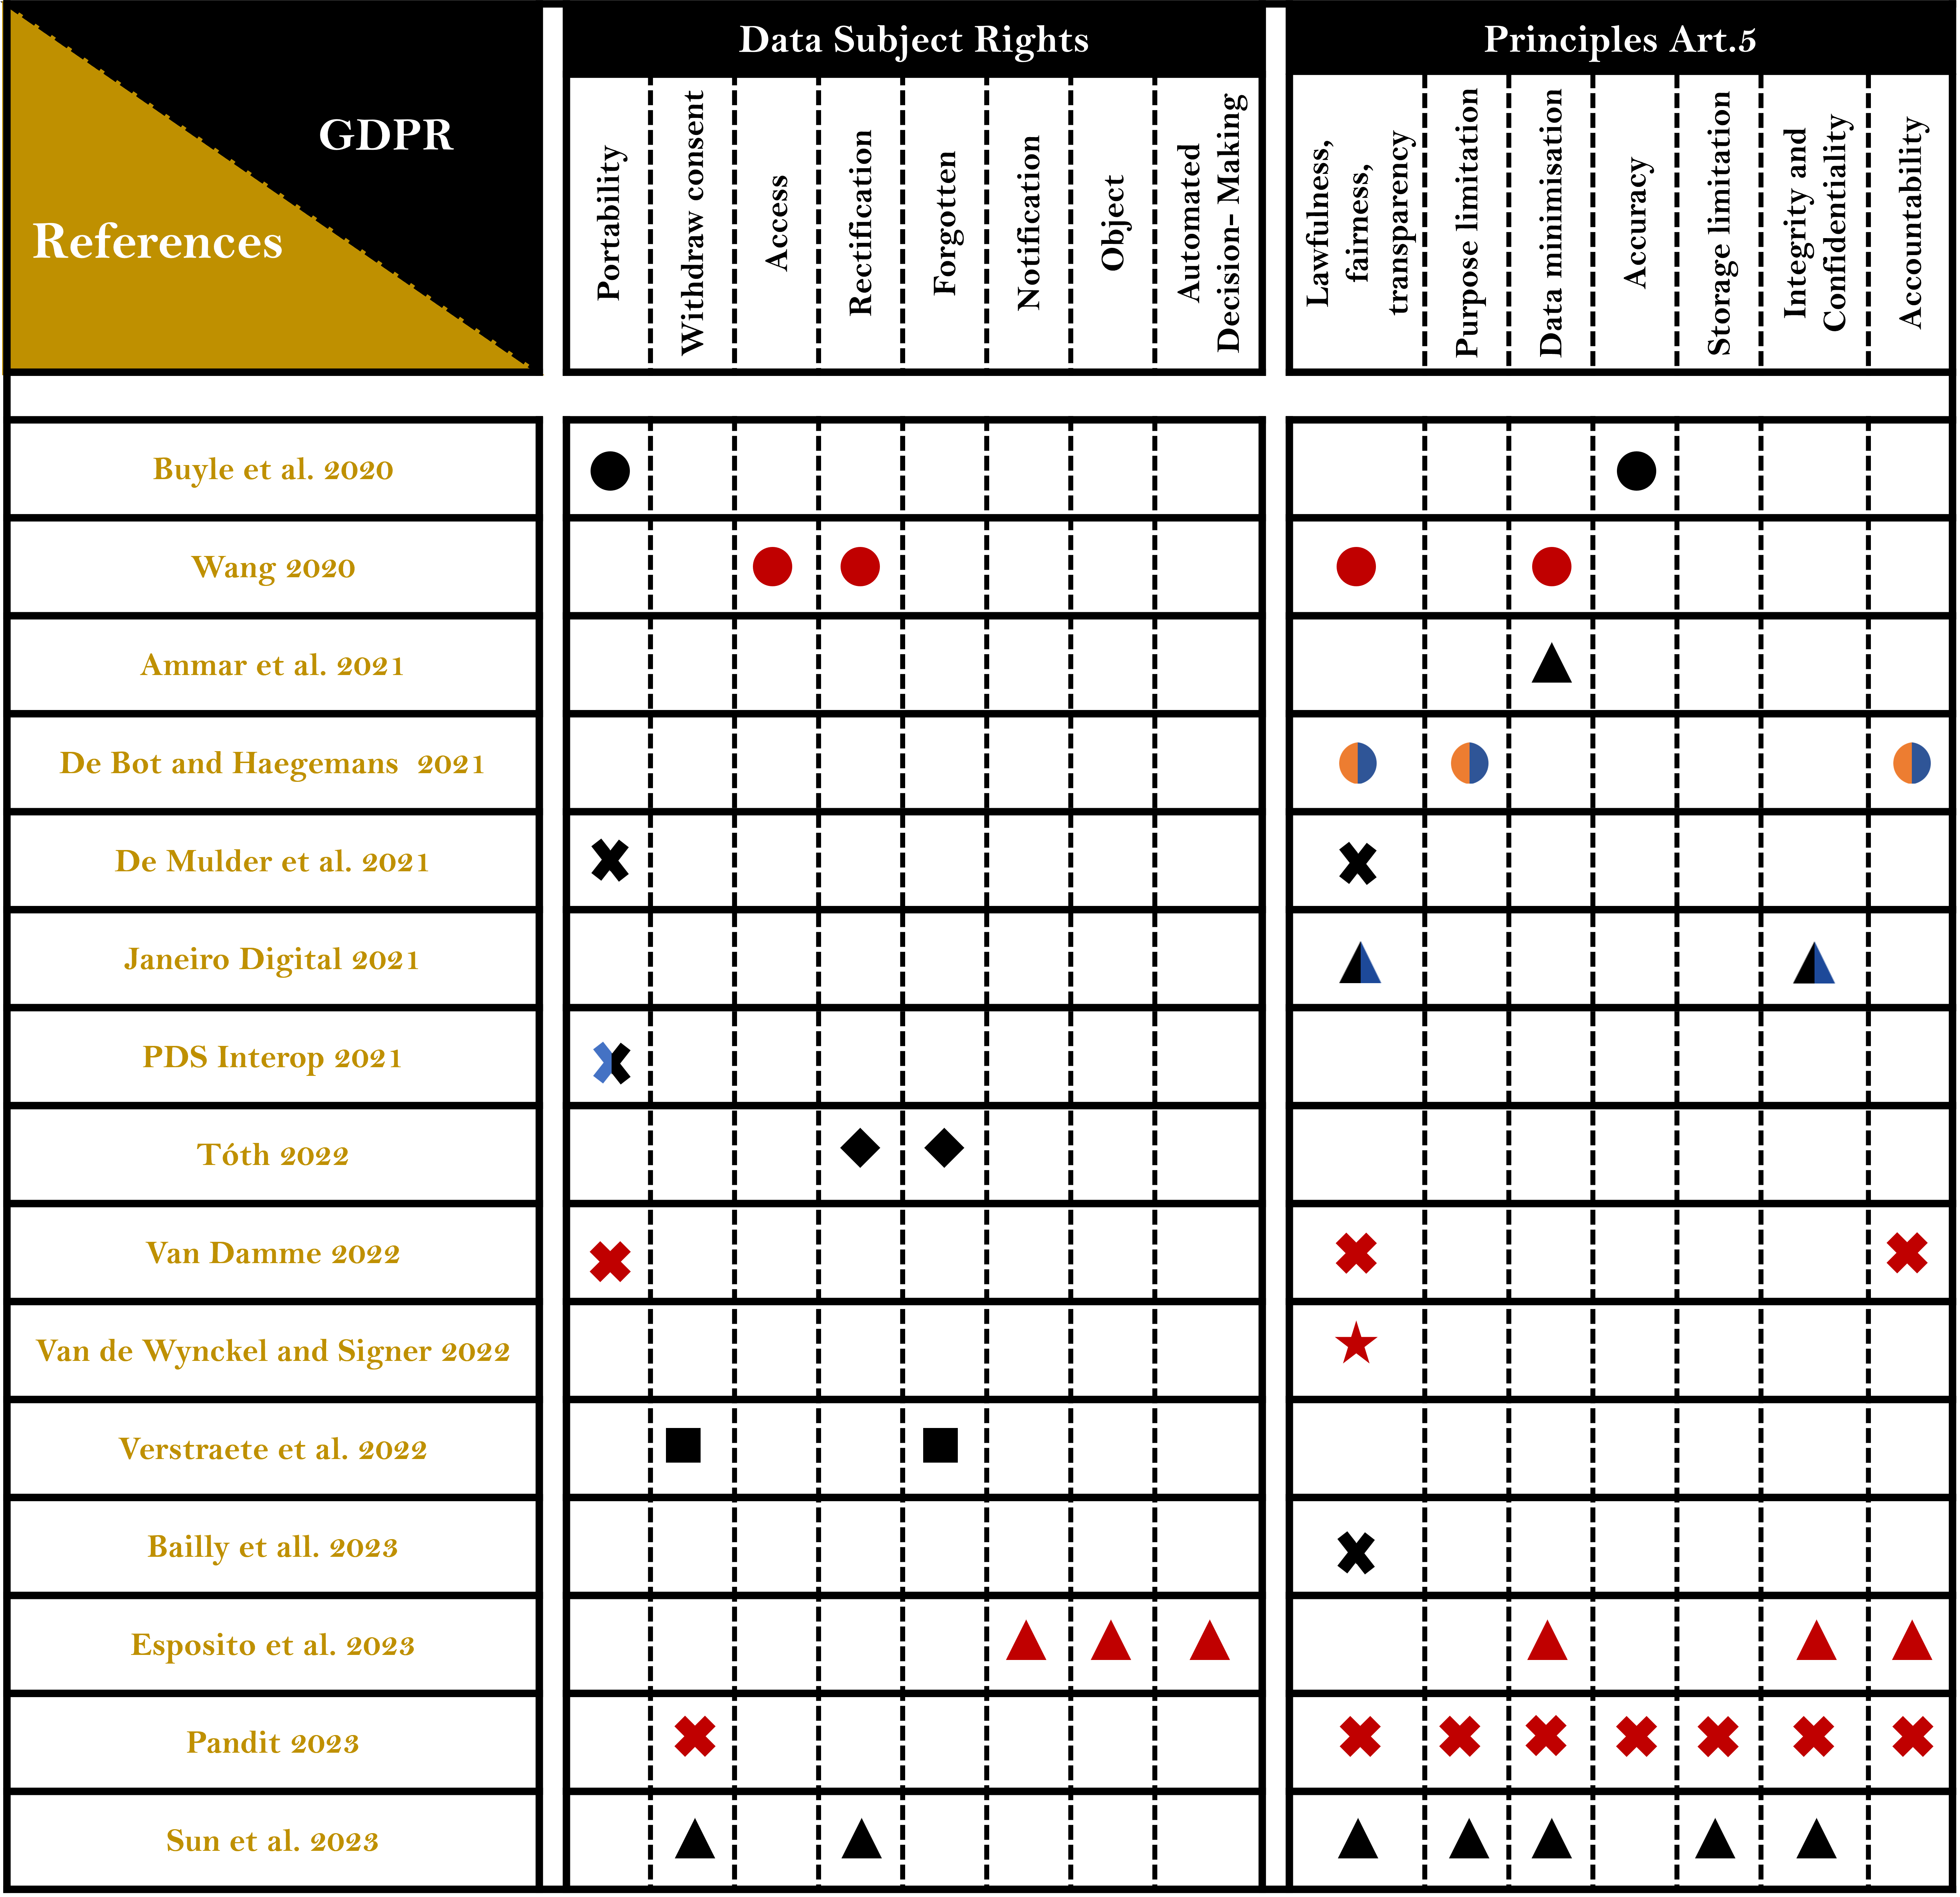
\includegraphics[width=\textwidth]{figures/chapter-2/solid-sota.png}
\caption[Comparison of existing work on Solid and data protection topics.]{Comparison of existing work on Solid and data protection topics. Each work was analysed in terms of whether it assists in the exercising of data subject rights or in the implementation of a certain GDPR principle, as well as the type of solution they developed -- works describing Solid apps are marked with a \textbf{black} shape, identity provider solutions with a \textbf{\textcolor{orange}{orange}} shape, Pod provider solutions with a \textbf{\textcolor{blue}{blue}} shape and theoretical work with a \textbf{\textcolor{red}{red}} shape. In addition, works marked with a $\medcircle$ discuss a government-related use case, $\medtriangleup$ a health-related use case, $\meddiamond$ a hospitality-related use case, \faStarO\space a location-related use case, $\medsquare$ a human resources-related use case and \textbf{X} represents work without a particular domain-related use case.}
\label{fig:solid_sota}
\end{figure}

As illustrated by the Figure, most works concentrate on fulfilling one or more GDPR principles, with a strong focus on the \textit{`lawfulness, fairness and transparency'} principle.
Distinct works were also found to tackle the right to data portability, withdrawal of consent, and rectification, while no specific work was found on the right to restrict the processing of personal data.

\subsection{Other decentralised technologies}
\label{sec:sota_other_technologies}

In addition to Solid and its stack of technologies, there is a set of tools and resources that support decentralisation and are either being discussed or should be discussed to be included in the Solid ecosystem.
We briefly present them in this Section as they should be considered in future research in this area.

\paragraph{Decentralised Identity}
The Decentralized identifiers (DIDs) data model is a recent W3C Recommendation that enables \textit{``individuals and organizations to generate their own identifiers using systems they trust''}~\citep{sporny_decentralized_2022}\footnote{A DID Solid method specification is in the early stages of development, with no official implementations being known to date -- available at \url{https://solid.github.io/did-method-solid/} (accessed on 19 August 2023).}.
In contrast with centralised settings, DIDs allow something or someone to be identified by a globally unique identifier which is detached from centralised registries, identity providers, or certificate authorities.
Moreover, DIDs work in a similar fashion to WebIDs -- DIDs are still URIs that can be dereferenced to return a DID document which \textit{``can express cryptographic material, verification methods, or services [...] to prove control of the DID''}.
The European Commission is also promoting the emergence of digital identity wallets for EU citizens, residents, and businesses to identify themselves, both online and offline, and to exchange certain types of personal identification data such as birth certificates or driving licenses.
In this context, the electronic IDentification, Authentication and trust Services (eIDAS) regulation~\citeyearpar{noauthor_regulation_2014}, and its amendment~\citeyearpar{noauthor_eidas2_2021}, puts forward \textit{``rules for trust services''} and \textit{``a legal framework for electronic signatures, electronic seals, electronic time stamps, electronic documents, electronic registered delivery services and certificate services for website authentication''}, while the 2021 amendment explicitly adds \textit{``conditions for the issuing of European Digital Identity Wallets''} and additional considerations derived from the GDPR.

\paragraph{Verifiable Credentials}
W3C's Verifiable Credentials (VCs) data model specification describes \textit{``a standard way to express credentials on the Web in a way that is cryptographically secure, privacy-respecting, and machine-verifiable''}~\citep{sporny_verifiable_2023}, using technologies such as digital signatures.
As in the physical world, VCs can be used to identify data subjects, to provide government-issued documents, e.g., ID cards or passports, or to deliver information on how the credential was created/derived and other constraints such as validity period or conditions for use.
An example of a VC, with a DID-identifiable subject, is presented in Listing \ref{list:vc_fromspec}.
The usage of VCs is being contemplated in the ACP specification, however, no specific details are provided regarding its implementation/development.

\begin{listing}[ht]
\caption[Verifiable credential with terms of use.]{Verifiable credential with terms of use where the issuer is prohibiting verifiers from archiving a degree credential, extracted from~\cite{sporny_verifiable_2023}, with the credential subject being identified by a DID.}
\label{list:vc_fromspec}
\begin{minted}{json}
{
    "@context": [
        "https://www.w3.org/ns/credentials/v2",
        "https://www.w3.org/ns/credentials/examples/v2"
    ],
    "id": "http://university.example/credentials/3732",
    "type": ["VerifiableCredential", "ExampleDegreeCredential"],
    "issuer": "https://university.example/issuers/14",
    "validFrom": "2010-01-01T19:23:24Z",
    "credentialSubject": {
        "id": "did:example:ebfeb1f712ebc6f1c276e12ec21",
        "degree": {
          "type": "ExampleBachelorDegree",
          "name": "Bachelor of Science and Arts"
        }
    },
    "termsOfUse": [{
        "type": "IssuerPolicy",
        "id": "http://example.com/policies/credential/4",
        "profile": "http://example.com/profiles/credential",
        "prohibition": [{
            "assigner": "https://university.example/issuers/14",
            "assignee": "AllVerifiers",
            "target": "http://university.example/credentials/3732",
            "action": ["Archival"]
        }]
    }] 
}
\end{minted}
\end{listing}

Moreover, \cite{braun_selfverifying_2022,braun_attributebased_2022} have previously published work on using VCs and RDF-star\footnote{RDF-star\citep{arndt_rdfstar_2023} is an under-development W3C specification that \textit{``extends RDF with a convenient way to make statements about other statements''}.} to sign and verify Web resources using a Solid app\footnote{The source code is available at \url{https://github.com/uvdsl/solid-web-ldsig}, under an MIT license (accessed on 19 August 2023).} and on using VCs and Linked Data Notifications (LDNs)\footnote{The W3C LDNs Recommendation \citep{capadisli_linked_2017} is a protocol that describes how servers can send and retrieve RDF-based messages, sent/retrieved by applications.}, extending previous work from~\citeauthor{ezike_solidvc_2019}, to request attribute-based access to Solid Pods\footnote{The source code is available at \url{https://github.com/uvdsl/solid-vc-pwa/}, under an MIT license (accessed on 19 August 2023).}.
\section{Representing personal data processing information}
\label{sec:sota_vocabularies}

The Web of Data and its semantic specifications are thriving, with the W3C guiding this effort to have machine-readable and interoperable linked data on the Web, described by open standards which promote portability and extensibility, allow for seamless integration of data from different origins and re-usage across distinct Web applications and services \citep{berners-lee_semantic_2001}.
Accordingly, a wave of vocabularies and ontologies has appeared in the last few years to formalise common concepts, such as objects or entities, or terms from specific domains, such as legal or medical ontologies.
More recently, with the increasing concerns around personal data processing abuse by Big Tech companies, data protection has been on the agenda of governments in a worldwide manner, with the EU taking the lead with its data protection law, the GDPR.
This has led to a new wave of personal data protection law ontologies being developed to help companies to comply with GDPR's legal requirements and which also intend to assist individuals to manage their personal data.

In the following Sections, the criteria used to analyse each specified data protection vocabulary are included, as well as a description of each identified solution.

\subsection{Criteria for analysis}
\label{sec:sota_vocabularies_criteria}

For each identified solution, we describe the core terms formalised in the ontologies, as well as dependencies on other existing works, and, when available, case studies where it has been applied.
As for the analysis of their representational abilities, we analyse whether such ontologies can represent the privacy terms mentioned in GDPR's data subject rights, to assess to what extent they can be used by data subjects to exercise their rights and by data controllers to manage compliance.

In particular, the so-called \textit{`right to be informed'}, described in detail on Articles 13 and 14, obliges data controllers to inform data subjects about any processing of personal data, whether being from data collected directly from the data subjects or from other sources. In addition to this, the following rights are also provided to data subjects:

\begin{enumerate}
  \item[(Art. 15)] \textit{`right of access'} to the personal data being processed, including a copy of the data as well as information about the purposes for processing, categories of the personal data being processed and their source, any recipients to whom the data may have been shared and corresponding measures to ensure its security, storage and retention conditions and the existence of other data subject's rights.
  \item[(Art. 16)] \textit{`right to rectification'} of inaccurate or incomplete personal data.
  \item[(Art. 17)] \textit{`right to be forgotten'}  by the data controllers when the personal data is no longer needed for the purposes for which it was collected.
  \item[(Art. 18)] \textit{`right to restriction of processing'} of personal data when its accuracy is being contested, the processing is unlawful, when the data subject needs it for any legal claims or objects to the processing.
  \item[(Art. 19)] \textit{`right to be notified'} about the rectification, erasure or restriction of processing.
  \item[(Art. 20)] \textit{`right to data portability'}, including the right to request that said data be transferred directly from one controller to another.
  \item[(Art. 21)] \textit{`right to object'} to any processing, including profiling.
  \item[(Art. 22)] \textit{`right to not be subjected to automated decision-making'}, including profiling.
\end{enumerate}

For such rights to be exercised by data subjects and fulfilled by data controllers, a set of privacy terms must be modelled, namely the terms identified in Table \ref{tab:GDPR_privacy_terms}, which is derived from \cite{esteves_analysis_2022}. These terms will be used to compare the described privacy and data protection vocabularies and ontologies and identify representational gaps in the existing solutions. The outcomes of this comparative analysis will be provided in Section \ref{sec:sota_vocabularies_analysis}.

\begin{table}
\centering
\caption{Privacy terms to be represented and respective identifiers (I*). The GDPR articles that mention these terms are also specified.}
\label{tab:GDPR_privacy_terms}
\resizebox{\textwidth}{!}{%
\begin{tabular}{c||l|c}
 I* & Informational Items & \textbf{GDPR Article(s)} \\
 \hline\hline
 I1 & Controller identity & \textbf{13.1(a), 14.1(a)} \\
 \hline
 I2 & Controller contact details & \textbf{13.1(a), 14.1(a)} \\
 \hline
 I3 & Controller's representative identity & \textbf{13.1(a), 14.1(a)} \\
 \hline
 I4 & Controller's representative contact details & \textbf{13.1(a), 14.1(a)} \\ 
 \hline
 I5 & DPO contact details & \textbf{13.1(b), 14.1(b)} \\
 \hline
 I6 & Purposes of the processing & \textbf{13.1(c), 14.1(c), 15.1(a)} \\ 
 \hline
 I7 & Legal basis of the processing & \textbf{6.1, 9.2, 13.1(c), 14.1(c)} \\ 
 \hline
 I8 & Legitimate interests & \textbf{6.1(f), 13.1(d), 14.2(b)} \\ 
 \hline
 I9 & Recipients / categories of recipients & \textbf{13.1(e), 14.1(e), 15.1(c), 17.2, 19} \\
 \hline
 I10 & Transfers to third countries & \textbf{13.1(f), 14.1(f)} \\ 
 \hline
 I11 & Retention period & \textbf{13.2(a), 14.2(a), 15.1(d)} \\ 
 \hline
 I12 & Data subject's rights & \textbf{13.2(b), 14.2(c), 15.1(e)} \\ 
 \hline
 I13 & Right to withdraw consent & \textbf{6.1(a), 9.2(a), 13.2(c), 14.2(d)} \\ 
 \hline
 I14 & Right to lodge a complaint & \textbf{13.2(d), 14.2(e), 15.1(f)} \\ 
 \hline
 I15 & Statutory or contractual obligation details & \textbf{13.2(e)} \\ 
 \hline
 I16 & Existence of automated decision making & \textbf{13.2(f), 14.2(g), 15.1(h), 22.1, 22.4} \\ 
 \hline
 I17 & Categories of personal data & \textbf{9.1, 14.1(d), 15.1(b)} \\ 
 \hline
 I18 & Source of personal data & \textbf{14.2(f), 15.1(g)} \\ 
 \hline
 I19 & Grounds to not comply with information right & \textbf{13.4, 14.5} \\
 \hline
 I20 & Safeguards related to the transfer to a third country & \textbf{15.2} \\ 
 \hline
 I21 & Copy of personal data & \textbf{15.3, 20.1} \\ 
 \hline
 I22 & Request to complete incomplete personal data & \textbf{16} \\ 
 \hline
 I23 & Grounds to request erasure of data & \textbf{17.1} \\ 
 \hline
 I24 &  Technical measures taken to erase data & \textbf{17.2} \\
 \hline
 I25 & Recipients contact details & \textbf{17.2, 19} \\
 \hline
 I26 & Grounds to not comply with right of erasure & \textbf{17.3} \\
 \hline
 I27 & Grounds to request restriction of processing & \textbf{18.1} \\
 \hline
 I28 & Transfer data directly between controllers & \textbf{20.2} \\
 \hline
 I29 & Grounds to not comply with right to object & \textbf{21} \\
 \hline
 I30 & \multicolumn{1}{l|}{\begin{tabular}[l]{@{}l@{}} Grounds to not comply with right not to be \\ subjected to decision making \end{tabular}} & \textbf{22.2} \\
\end{tabular}}
\end{table}

\subsection{Personal data protection vocabularies}
\label{sec:sota_vocabularies_description}

% TODO: https://openscience.adaptcentre.ie/ontologies/GConsent/docs/ontology#related-work 

In this Section, a systematic description of each identified work is provided, including an example that uses the vocabulary's concepts, when available.
Moreover, Table \ref{tab:analysed_vocabularies} provides an overview of these solutions and supplies information about the creators of the resources, their versions, the date of publication and the date of the last known update.
Said solutions are then analysed in chronological order regarding the date of publication and a dependency graph -- a chart that demonstrates the relations between the reviewed vocabularies and its dependencies and extensions -- is presented in Figure \ref{fig:voc_dependency_graph}.

\begin{table}
\centering
\caption{Brief description of the vocabularies described in Section \ref{sec:sota_vocabularies_description}.}
\label{tab:analysed_vocabularies}
\resizebox{\textwidth}{!}{%
\begin{tabular}{c||c|c|c|c|c}
Abbreviation (Section) & Full Name & Creators & Version & \multicolumn{1}{c|}{\begin{tabular}[c]{@{}c@{}} Date of \\ publication \end{tabular}} & \multicolumn{1}{c}{\begin{tabular}[c]{@{}c@{}} Last \\ update \end{tabular}} \\
 \hline\hline
 \multicolumn{1}{c||}{\begin{tabular}[c]{@{}c@{}} DPKO, \\ DPRO (\ref{sec:neurona}) \end{tabular}} & \multicolumn{1}{c|}{\begin{tabular}[c]{@{}c@{}} Data Protection Knowledge Ontology, \\ Data Protection Reasoning Ontology \end{tabular}} & Casellas et al. & - & 2008 & 2010 \\
 \hline
 DPO (\ref{sec:dpo}) & Data Protection Ontology & Bartolini and Muthuri & - & 2015 & 2016 \\
 \hline
 GDPRov (\ref{sec:gdprov}) & GDPR Provenance Ontology & Pandit and Lewis & 0.7 & 2017 & 2019 \\
 \hline
 Cloud (\ref{sec:cloud}) & Cloud GDPR ontology & Elluri and Joshi & - & 2018 & - \\
 \hline
 PrOnto (\ref{sec:pronto}) & Privacy Ontology for legal reasoning & Palmirani et al. & - & 2018 & - \\
 \hline
 GConsent (\ref{sec:gconsent}) & GDPR Consent ontology & Pandit et al. & 0.5 & 2018 & - \\
 \hline
 IMO (\ref{sec:imo}) & Information Model Ontology & Lioudakis and Cascone & 1.0 & 2018 & - \\
 \hline
 DPV (\ref{sec:dpv}) & Data Privacy Vocabulary & Pandit et al. & 1.0 & 2018 & 2022 \\
 \hline
 \hline
 GDPRtEXT (\ref{sec:gdprtext}) & GDPR text EXTensions & Pandit et al. & 0.7 & 2018 & 2020 \\
\end{tabular}}
\end{table}

\begin{figure}
\caption{Data protection vocabularies dependency chart.}
\label{fig:voc_dependency_graph}
\centering
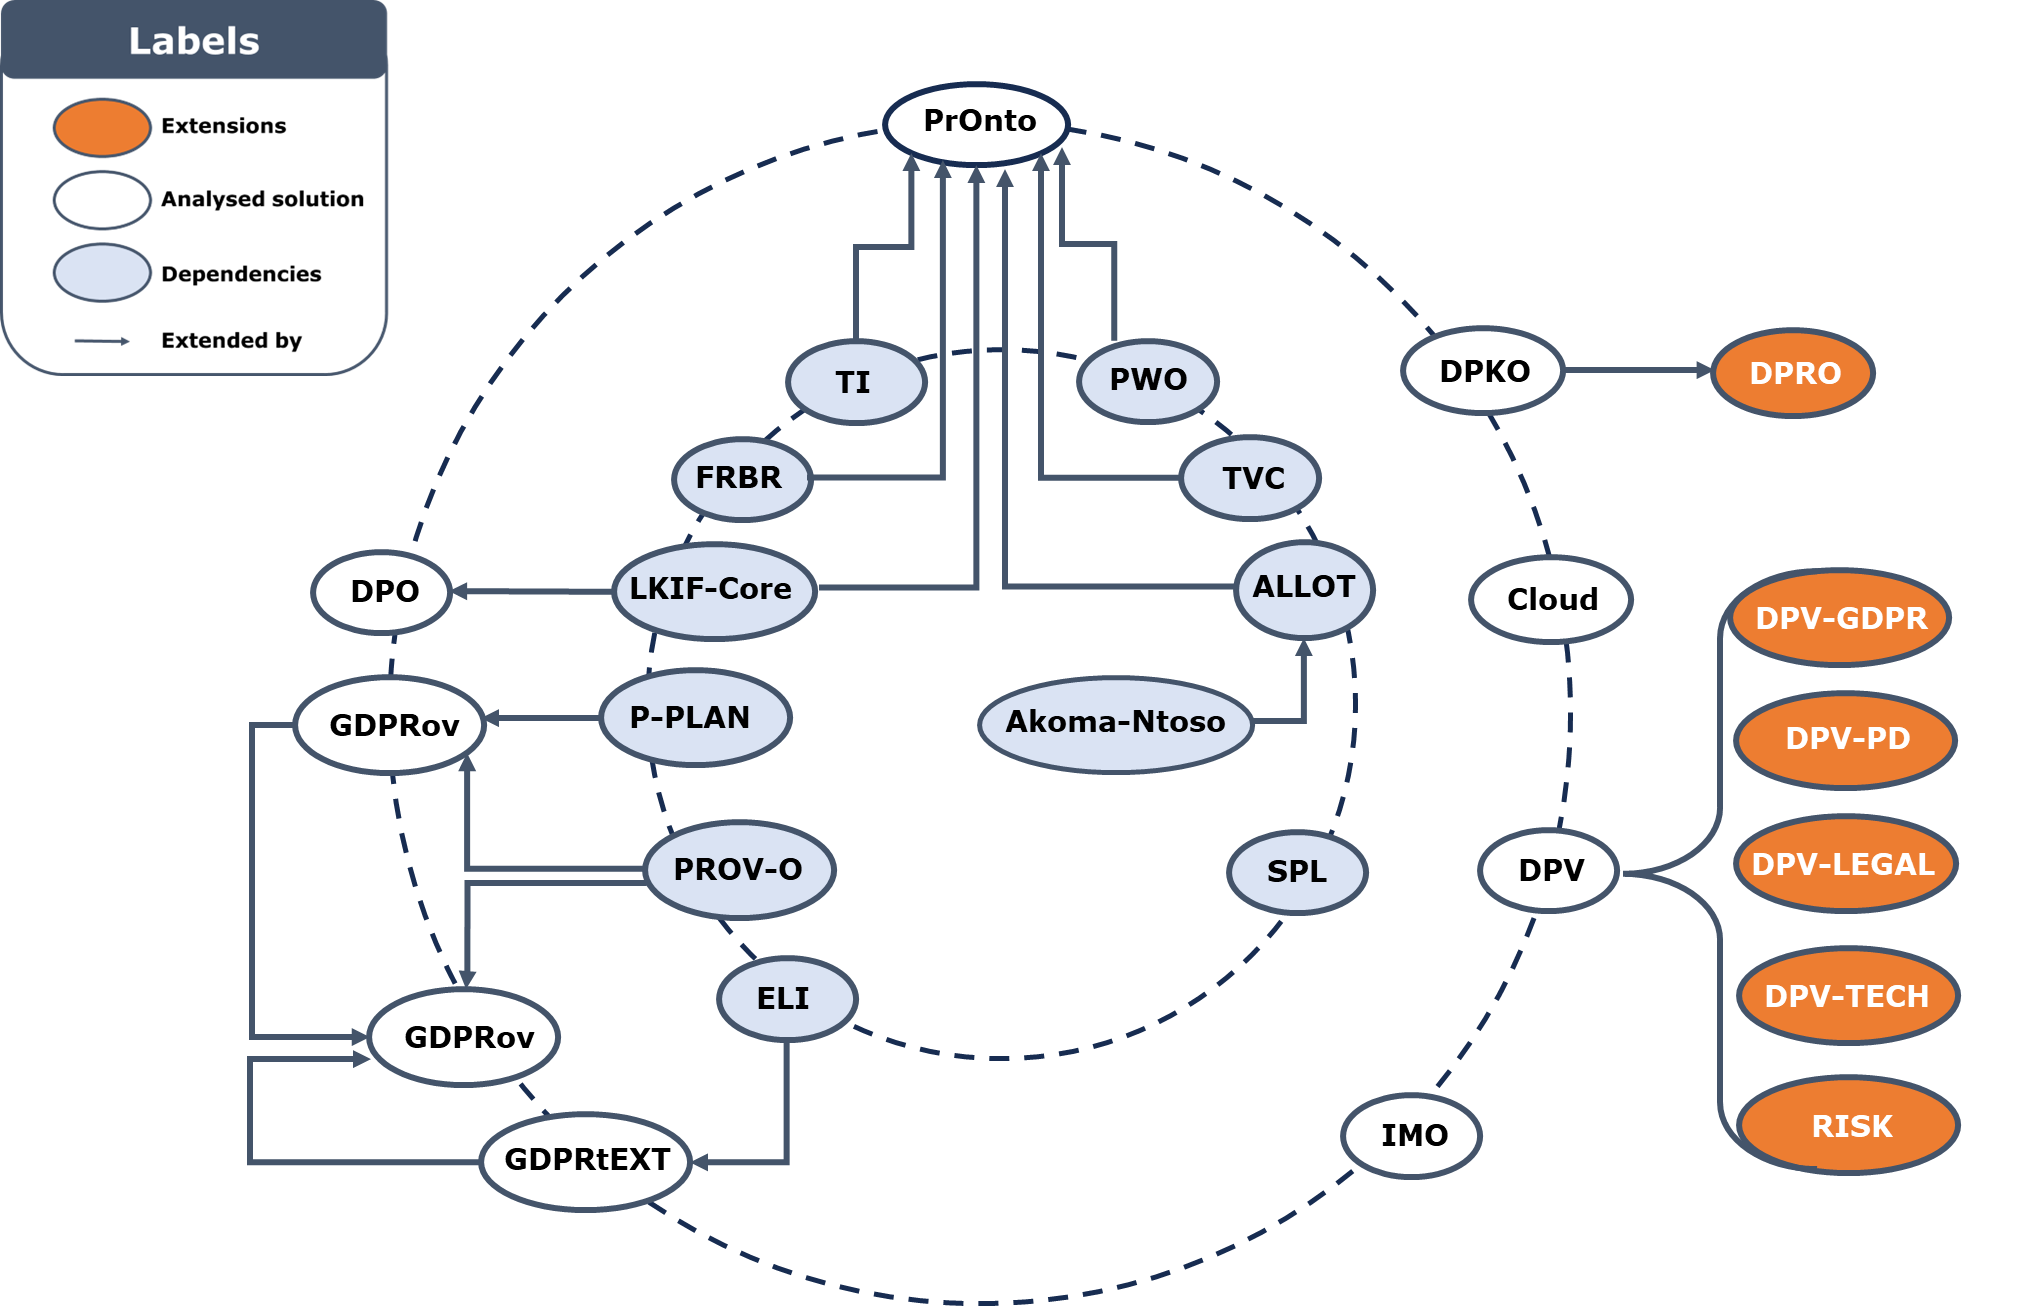
\includegraphics[width=\textwidth]{figures/chapter-2/vocabs.png}
\end{figure}

To complement the description of vocabularies presented in this Section, additional documentation and resources were published in a Web page\footnote{Available at \url{https://protect.oeg.fi.upm.es/sota/ontologies}. Its public repository can be consulted at \url{https://github.com/besteves4/SotAResources} for further improvement when new solutions appear.}, including diagrams and code examples.

\subsubsection{NEURONA}
\label{sec:neurona}

The NEURONA project \citep{casellas_ontological_2010}, developed by S21SEC\footnote{\url{https://www.s21sec.com/} (accessed on 16 July 2023)} and IDT-UAB\footnote{\url{https://portalrecerca.uab.cat/en/organisations/law-and-technology-institute} (accessed on 16 July 2023)}, created two ontologies based on the pre-GDPR Spanish personal data protection regulation \citeyearpar{noauthor_real_2008} -- the Data Protection Knowledge Ontology (DPKO) and the Data Protection Reasoning Ontology (DPRO).
These ontologies are, however, not publicly available for re-usage.

The main objectives of the ontologies developed in the context of this project were to represent security measures for files containing personal data and reason over their correctness.
DPKO's main classes are \textbf{data}, \textbf{consent}, \textbf{purpose}, \textbf{person}, \textbf{security measures} and \textbf{security degree}.
In relation to the data class, categories such as health data are defined and associated with special security measures. 
The consent should be given by the data subject in an unambiguous way and for a specific purpose.
In addition, technical and organisational measures (TOMs) for data security, such as access control measures or authentication procedures, are modeled and connected to the nature of the data, taking into consideration the security level associated with the type of data or how the data was obtained. 
For example, a file with health data obtained without consent should have high-level security measures, while a file with anonymised data can implement low-level measures.
DPRO is then used to access data protection compliance by reasoning over the measures applied to files.

\subsubsection{DPO}
\label{sec:dpo}

The Data Protection Ontology (DPO) \citep{bartolini_reconciling_2015,otake_using_2017} concentrates on the modelling of data protection principles and data controller obligations. It is based on an early version of the GDPR, prior to its implementation in May 2018, on the Data Protection Directive \citeyearpar{noauthor_directive_1995} and the \textit{Handbook on European data protection law} \citep{european_union_agency_for_fundamental_rights_and_council_of_europe_handbook_2018} and reuses concepts from the LKIF-Core \citep{hoekstra_lkif_2007} ontology.

The core classes of DPO are \textbf{data protection principles}, \textbf{rules} for processing and transferring data, and \textbf{data subjects rights}.
The ontology is designed so that each rule and right is linked to at least one principle.
For instance, data subjects have the right to rectify inaccurate or incomplete data and data controllers must provide the means to do it, according to GDPR's \textit{`accuracy'} principle.
Furthermore, DPO defines consent as a legal justification connected with the principle of trust and also specifies concepts to model the special case of giving consent as a parent for a child, although the concept of \textit{`consent provided by delegation'} is missing.
Data protection-related entities, such as data controllers, supervisory authorities, processors, representatives or data protection officers, are modelled as a type of \textbf{person}.

Listing \ref{list:sparql_dpo} provides an example of a SPARQL query to retrieve duties of a data controller that do not concern the transfer of personal data using DPO.\footnote{More examples are available in a project repository at \url{https://bitbucket.org/guerret/lu.uni.eclipse.bpmn2/} (accessed on 16/July/2023).}

\begin{listing}
\caption{SPARQL query to retrieve duties of the data controller that do not concern data transfer using the Data Protection Ontology.}
\label{list:sparql_dpo}
\begin{minted}{sparql}
SELECT DISTINCT ?duty WHERE {
    ?x rdfs:subClassOf* [ rdf:type dpo:Rule ] .
	?x rdfs:label ?duty
	MINUS {
		?x rdfs:subClassOf* [ rdf:type dpo:TransferRule ] .
		?x rdfs:label ?duty .
	} .
	FILTER (?duty != "Rule"@en && ?duty != "ProcessingRule"@en && ?duty != "TransferRule"@en) }
\end{minted}
\end{listing}

\subsubsection{GDPRov}
\label{sec:gdprov}

The GDPR Provenance Ontology (GDPRov) \citep{pandit_modelling_2017} aims to record the provenance of personal data and of the consent conditions and processing activities performed over such data, according to the GDPR.
GDPRov extends PROV-O \citep{lebo_prov-o_2013}, a W3C Recommendation created to define the provenance of entities and systems, and P-Plan \citep{garijo_augmenting_2012}, an extension of PROV-O to represent activities and corresponding steps to execute them, as well as the entities involved.
Using these terms, it is possible to monitor changes in consent or to track the interaction between entities involved in the exchange of data.

GDPRov's main concept to record the provenance of consent is the \textbf{consent agreement template} class, a common template which includes the consent conditions presented to the users and the entities in charge of data  processing, and also information on third party sharing, approved processing activities and additional rights.
Provenance metadata on the origin, use, storage and sharing of the data can also be recorded with GDPRov, as well as information regarding transformations performed to the data.
In addition to this, provenance data on the exercising and fulfilment of GDPR-related rights and obligations can also be represented with GDPRov -- for each right or obligation, a plan can be modelled to include the activities that need to be executed when an user exercises a particular right.

Listing \ref{list:sparql_gdprov} illustrates a SPARQL query which uses GDPRov's terms to retrieve the entities involved in acquiring consent.

\begin{listing}
\caption{SPARQL query retrieving entities involved in acquiring consent using GDPRov \citep{pandit_modelling_2017}.}
\label{list:sparql_gdprov}
\begin{minted}{sparql}
SELECT ?consent ?template ?toc WHERE {
    ?consent a gdprov:ConsentAgreement .
    ?template a gdprov:ConsentAgreementTemplate .
    ?toc a gdprov:TermsAndConditions .
    ?step a gdprov:ConsentAcquisitionStep .
    ?step gdprov:usesConsentAgreementTemplate ?template .
    ?step gdprov:usesTermsAndConditions ?toc .
    ?step gdprov:generatesConsentAgreement ?consent }
\end{minted}
\end{listing}

\subsubsection{Cloud}
\label{sec:cloud}

The Cloud GDPR ontology was developed by \cite{elluri_knowledge_2018} to express data protection obligations of cloud data consumers and providers, taking into consideration the Cloud Security Alliance (CSA) controls defined on the \textit{Code of Conduct for GDPR Compliance} \citep{cloud_security_alliance_-_privacy_level_agreement_working_group_code_2017}.

The \textbf{stakeholders}, \textbf{controls} and \textbf{obligations} are the core concepts of this ontology.
Cloud-related obligations are extracted and connected to GDPR's articles and are also associated to CSA requirements using the \textbf{hasCSAcontrol} property.
Moreover, these obligations are further specified into common or provider/consumer-specific obligations taking into consideration which stakeholders they are applicable to, e.g., maintaining records of data processing activities and notifying data breaches are common obligations, while providing legal representatives for non-EU stakeholders or hiring a DPO are the responsibility of the consumer and of the provider, respectively.

This work was later extended \citep{elluri_integrated_2018} to automate the implementation of compliance tasks mandated by the GDPR and the Payment Card Industry Data Security Standard (PCI DSS) guidelines \citep{pci_security_standards_council_payment_2018} and also to include the rights of consumers, providers and end users.
These guidelines deal with financial data, such as the credit card number or card-holder's name, which fall under the protection offered by the GDPR.
As such, and since its scope is narrower, a data breach of PCI DSS-related data automatically results in GDPR-related one.
Thus, the cloud-related PCI DSS requirements were used to enhance this ontology and its evaluation was performed using privacy policies from five major companies that deal with card-holder's data.

\subsubsection{PrOnto}
\label{sec:pronto}

PrOnto, the Privacy Ontology for legal reasoning, aims to model GDPR-related associations between agents, processing activities, data categories and deontic modalities, with the main goal to support legal reasoning and compliance with data protection regulations \citep{ko_pronto_2018}.
PrOnto relies on a number of ontologies to model these relationships:
\begin{itemize}
    \item LKIF-Core \citep{hoekstra_lkif_2007} is used to model agents, e.g., organisations, software or people, as well as the several legal roles which can be assigned to them, i.e., acting as a data controller or processor.
    \item The Functional Requirements for Bibliographic Records (FRBR) ontology \citep{byrum_functional_2009} is used to model legal documents as sources of information, that regulate the different relationships between the agents documented in the text, and to register changes in their representation over time. % copied
    \item The ALLOT (A Light Legal Ontology On Top level classes) ontology, developed by Barabucci et al. \citep{barabucci_managing_2010}, extends the Akoma Ntoso standard \citep{palmirani_akoma-ntoso_2011} to link documents with the data they contain, e.g., people, events or locations.
    \item The Publishing Workflow Ontology (PWO) \citep{gangemi_publishing_2017} is used to characterize provenance data associated with the publication of a document, e.g., to model the different types of processing of personal data.
    \item The TVC (Time-indexed Value in Context) ontology \citep{peroni_semantic_2014} and the TI (Time Interval) ontology pattern\footnote{\url{http://www.ontologydesignpatterns.org/cp/owl/timeinterval.owl} (accessed on 16/July/2023)} are used to associate time-dependant variables such as events to specific agent roles that only emerge in particular point in time.
\end{itemize}

PrOnto's main classes are defined as follows: \textbf{documents and data}, \textbf{agents and roles}, \textbf{processing and workflow}, \textbf{legal rules and deontic formula}, and \textbf{purposes and legal bases}.
GDPR is the main document used to extract personal data categories such as judicial or sensitive data and non-personal data such as anonymous or legal person data.
Moreover, processing activities are represented as a workflow of actions that should be recorded together with provenance data such as the context and time in which each action occurs.
Each processing activity is also associated with a purpose and a legal rule, which is composed of deontic specifications, i.e., prohibitions, rights, permissions and obligations, used to check if the activity being executed is compliant with the GDPR. PrOnto is, however, not publicly available for re-usage, which hinders the assessment of the totality of concepts it models\footnote{As PrOnto is not available online, its namespace is unknown. We use the prefix \texttt{pronto} to identify PrOnto's concepts that are available in the analysed publication.}. 

Listing \ref{list:sparql_pronto} illustrates a query to retrieve information regarding personal data processing activities performed by company X in the role of controller from time t1 to t2.

\begin{listing}
\caption{SPARQL query used to retrieve personal data processing activities performed by company X in the role of controller from t1 to t2 using PrOnto \citep{ko_pronto_2018}.}
\label{list:sparql_pronto}
\begin{minted}{sparql}
SELECT ?pdp WHERE {
    ?pdp pronto:isManagedBy _:c .
    [ lkif:plays _:c ;
        rdfs:label "X" ] .
    ?pdp pronto:isValid [
        ti:hasIntervalStartDate [ 
            a ti:TimeInterval; rdfs:label "t1" ] ;
        ti:hasIntervalEndDate [ 
            a ti:TimeInterval; rdfs:label "t2" ] ] . }
\end{minted}
\end{listing}

\subsubsection{GConsent}
\label{sec:gconsent}

GConsent \citep{hitzler_gconsent_2019} is an ontology focused on the GDPR concept of consent and, as such, it models information regarding how consent was collected and stored, as well as records of any changes that may occur over time, including withdrawal, including data on the parties involved, according to Article 6 of the GDPR.
Additionally, other documentation sources were also adopted, including EDPB's guidelines on consent \citep{european_data_protection_board_guidelines_2020}.
As GConsent aims at not only capturing the concept of consent, but also to represent its state, context and provenance, existing vocabularies on this subject, such as PROV-O \citep{lebo_prov-o_2013}, GDPRov \citep{pandit_modelling_2017} and GDPRtEXT \citep{gangemi_gdprtext_2018} -- later presented in Section \ref{sec:gdprtext}, are reused. % copied

GConsent's main concepts are the terms to represent \textbf{data subjects}, \textbf{personal data}, \textbf{purpose} and \textbf{processing types}, as well as the \textbf{consent} and \textbf{consent status} classes -- the latter fills a gap on the available ontologies on this domain as it not only defines \textbf{explicitly given consent} as a concept, but also classifies other states of consent, such as \textbf{implicitly given}, \textbf{expired} or \textbf{refused}.
GConsent also includes concepts to represent information regarding the context in which the consent was obtained -- information about the entities involved, spatial and temporal aspects and the format used to record it, e.g., Web form, voice recording or signature -- and a taxonomy of processing types, e.g., data alignment or data retrieval.

Listing \ref{list:ttl_gconsent} provides an example of a record of provenance data regarding an activity of withdrawing consent using GConsent.

\begin{listing}
\caption{Turtle record of provenance data regarding an activity of withdrawing consent using GConsent \citep{hitzler_gconsent_2019}.}
\label{list:ttl_gconsent}
\begin{minted}{turtle}
_:modifyConsent a gdprov:ModifyConsentActivity ;
    prov:invalidated _:consent1 ;
    prov:generated _:consent2 .

_:consent1 a gc:Consent ;
    gc:isPreviousConsentFor _:consent2 ;
    gc:hasStatus gc:ConsentStatusExplicitlyGiven .

_:consent2 a gc:Consent ;
    gc:hasStatus gc:ConsentStatusWithdrawn .
\end{minted}
\end{listing}

\subsubsection{IMO}
\label{sec:imo}

The Information Model Ontology (IMO) \citep{papagiannakopoulou_leveraging_2014,lioudakis_compliance_2019} was developed in the context of the BPR4GDPR project\footnote{BPR4GDPR (Business Process Re-engineering and functional toolkit for GDPR compliance) is an European Union H2020 innovation programme with the main goal of providing a framework to reinforce the implementation of GDPR-compliant measures inside organizations at diverse scales and in several domains. More information available at \url{https://www.bpr4gdpr.eu/} (accessed on 16/July/2023).} and it aims to define the entities and respective roles that are involved in the organisation lifecycle of processing personal data.

IMO's core classes are \textbf{data types}, \textbf{roles} assigned to users within different \textbf{organization types}, \textbf{machine types} that host \textbf{operations} for particular \textbf{purposes}, \textbf{events} and their \textbf{context} information.
The roles class is related to the responsibilities that are assigned to the user in the context of the organization and its instances can be implemented hierarchically according to the detail level of the data and connected through the \textit{isA} property -- a structure which is valid for most classes in the ontology. % copied
The data processing activities are implemented through the operations class, which have associated the \textit{hasInput} and \textit{hasOutput} properties that allow to connect the operations with the data that is processed and the one that is generated and respective states, i.e., plain or anonymised. % copied
These operations can be grouped in an operation container -- a class that groups processing activities in contexts where they usually work together, for instance, in the management of a database, in which functions such as create, read, update or delete are commonly used.  % copied
The roles and operations classes should always be connected with an instance of the purpose class.  % copied
The events class, that aims at capturing all processing activities, a data breach or the revoke of consent, has associated the context class to instantiate specific cases and provide temporal and spatial details, among others.  % copied

% TODO: extract example from https://www.researchgate.net/profile/Joaquin-Garcia-Alfaro/publication/260706010/figure/fig3/AS:296857856167938@1447787836426/Example-of-Ontological-Access-Control-Rule.png

\subsubsection{DPV}
\label{sec:dpv}

The Data Privacy Vocabulary is being developed and maintained by the W3C Data Protection Vocabularies and Controls Community Group (DPVCG)\footnote{\url{https://www.w3.org/community/dpvcg/} (accessed on 16/July/2023)} -- an output of a W3C workshop on data privacy controls which took place in 2018, with the objective of defining priorities for the standardization of this domain \citep{bonatti_data_2018}.

DPV's core concepts, \textbf{processing}, \textbf{purpose}, \textbf{recipient} and \textbf{personal data categories}, were adapted from the SPECIAL Usage Policy Language (SPL) vocabularies \citep{bonatti_policy_2018} and new concepts were/are continuously added to DPV after being discussed and agreed upon by the Community Group.
In addition to previously mentioned concepts, DPV's base vocabulary was first published with the following additional classes: \textbf{legal basis}, \textbf{technical and organizational measures} and \textbf{legal entities}, including \textbf{data subject} and \textbf{child}, \textbf{recipients}, \textbf{data controller}, \textbf{data processor} and \textbf{third party} \citep{panetto_creating_2019}.
In December of 2022, DPV version 1 was published including additional concepts to model \textbf{risk}, \textbf{rights} and \textbf{data subject rights}, \textbf{technology}, \textbf{laws} and \textbf{context of processing} classes and the previously existing taxonomies were extended with new terms -- new legal entities, including authority and data protection authority, vulnerable data subject, data sub-processor, data protection officer and representative, were added to the vocabulary, as well as new purpose and legal basis sub-classes.
For instance, the purpose taxonomy is composed of 76 purpose sub-classes, which are topped by classes such as R\&D or Service Provision, and can be further constrained to specific contexts or business sectors, and DPV's processing operations taxonomy covers the terms defined in Article 4.2 of the GDPR, providing a set of 44 processing categories.

DPV also provides five extensions:
\begin{itemize}
    \item Personal data categories are defined in the DPV-PD extension\footnote{\url{https://w3id.org/dpv/dpv-pd} (accessed on 17/July/2023)} -- the personal data class is split into generic classes such as financial or social data, adapted from the \textbf{EnterPrivacy} taxonomy by \cite{cronk_categories_2017}, which are further specified into concepts such as credit card number or social media accounts.
    \item GDPR-specific concepts are defined in the DPV-GDPR extension\footnote{\url{https://w3id.org/dpv/dpv-gdpr} (accessed on 17/July/2023)} -- it covers legal bases specified on GDPR's Articles 6 and 9 for the processing of personal data and also the legal bases for the transfer of personal data to third countries defined on Articles 45, 46 and 49. It also models GDPR's data subject rights, data transfer tools and Data Protection Impact Assessment (DPIA) terms.
    \item Technology-relevant concepts are defined in the DPV-TECH extension\footnote{\url{https://w3id.org/dpv/dpv-tech} (accessed on 17/July/2023)} -- it includes concepts to model specific technologies, their management, technology actors and relevant tools and systems.
    \item Jurisdiction-relevant concepts are defined in the DPV-LEGAL extension\footnote{\url{https://w3id.org/dpv/dpv-legal} (accessed on 17/July/2023)} -- it contains terms related to specific laws, adequacy decisions and a taxonomy of authorities.
    \item Risk concepts are defined in the RISK extension\footnote{\url{https://w3id.org/dpv/risk} (accessed on 17/July/2023)} -- it covers concepts related to risk, likelihood, severity levels, consequences and impacts, as well as risk assessment techniques and methodologies.
\end{itemize}

Listing \ref{list:ttl_dpv} provides an example of a personal data handling related to the collection and usage of email addresses for marketing purposes using DPV.

\begin{listing}
\caption{Turtle record of a personal data handling related to the collection and usage of email addresses for marketing purposes using DPV \citep{panetto_creating_2019}.}
\label{list:ttl_dpv}
\begin{minted}{turtle}
_:AcmeMarketing a dpv:PersonalDataHandling ;
    dpv:hasDataController [ a dpv:DataController ] ;
    dpv:hasPersonalData dpv-pd:EmailAddress ;
    dpv:hasProcessing dpv:Collect, dpv:Use ;
    dpv:hasPurpose dpv:Marketing .
\end{minted}
\end{listing}

\subsubsection{GDPRtEXT}
\label{sec:gdprtext}

GDPRtEXT was developed by \cite{gangemi_gdprtext_2018} as a linked data resource, which extends the European Legislation Identifier (ELI) ontology \citep{office_of_publications_on_eur-lex_eu_2017}, to connect GDPR concepts with the specific chapters, articles or points of the regulatory text.

The main concepts modelled in this ontology are related to the specific \textbf{entities} mentioned in the GDPR text, their \textbf{rights} and \textbf{obligations}, the \textbf{principles} and the \textbf{activities} which specify processes and actions defined in the GDPR, such as reporting a data breach, exercising rights or demonstrating consent.
These terms are linked to the relevant GDPR articles using the \textbf{rdfs:isDefinedBy} property.

\subsection{Comparative analysis}
\label{sec:sota_vocabularies_analysis}

% TODO: \beatriz{DPKO: I7 - only consent; I17 - data}
% TODO: \beatriz{DPKO: I20 - transfer rule}

As it is visible in Tables \ref{tab:vocabsTerms-first} and \ref{tab:vocabsTerms-second}, existing ontologies and vocabularies in the domain of data protection are of particular interest to represent the privacy terms described in Table \ref{tab:GDPR_privacy_terms}, however, there are still representational gaps to be filled.
More specifically, each ontology was analysed in terms of the concepts they model and, when a particular concept was found to represent a particular privacy term, the name of the respective term was included in the comparative tables, as well as the number of sub-classes which can be used to more precisely define the term.
The cases in which there was no specific concept to represent the privacy term, yet there were terms that can be extended to accomplish it, are marked with an asterisk. % copied
Privacy terms I15, I19, I24, I26, and I28 to I30 are not represented in either Table \ref{tab:vocabsTerms-first} or \ref{tab:vocabsTerms-second} since they are not modeled by any of the analysed ontologies. % copied

DPO, GDPRov, PrOnto, DPV and GDPRtEXT can be used to partially populate a great deal of the informational items required by the \textit{`right to be informed'} and the other GDPR rights. % copied
However, DPV and GDPRtEXT must be highlighted since they contain the concepts to represent, at least partially, 19 and 14 privacy terms, respectively, out of the 30 described in Table \ref{tab:GDPR_privacy_terms}.
Furthermore, these vocabularies are the ones that have the largest number of sub-classes to specifically define the respective terms. % copied

Of particular importance, it must be referred that most of presented resources are obsolete or without new developments in recent years, with DPV being the only one that presented new outcomes in the last two years.
Moreover, of all the covered vocabularies, only DPKO, IMO and PrOnto do not have open and accessible resources. % copied

\begin{table}
\centering
\caption[Representation of privacy terms I1 to I22 in the DPKO, DPRO, DPO, GDPRov, Cloud and PrOnto ontologies.]{Representation of privacy terms I1 to I22 in the DPKO, DPRO, DPO, GDPRov, Cloud and PrOnto ontologies. The names of the classes which can be used to specify a particular item are depicted in the table, as well as their respective number of sub-classes, if available. The privacy terms which can not be fully represented by the current ontology terms are illustrated with an asterisk.}
\label{tab:vocabsTerms-first}
\resizebox{\textwidth}{!}{%
\begin{tabular}{ c||c|c|c|c|c|c}
 & DPKO & DPRO & DPO & GDPRov & Cloud & PrOnto \\
 \hline\hline
 I1 & & & Controller & Controller & & $\ast$ \\
 \hline
 I3 & & & & ControllerRepresentative & Identify\_Representatives & \\
 \hline
 I6 & Purpose & & Purpose & & & Purpose (10) \\
 \hline
 I7 & $\ast$ & & LegalJustification (6) & & & \\
 \hline
 I8 & & & LegitimateInterest & & & \\
 \hline
 I9 & & & Recipient (2) & & & $\ast$ \\
 \hline
 I10 & & & & $\ast$ & & \\
  \hline
 I11 & & & & & & $\ast$ \\
 \hline
 I12 & & & DataSubjectRight (7) & Process (10) & & Right (8) \\
 \hline
 I16 & & & AutomatedProcessing & $\ast$ & & \\
 \hline
 I17 & $\ast$ & & PersonalData & PersonalData (3) & & PersonalData (7) \\
 \hline
 I20 & & & $\ast$ & & & \\
 \hline
 I21 & & & & ProvideCopyOfPersonalData & & \\
 \hline
 I22 & & & & RectifyData & & \\
\end{tabular}}
\end{table}

\begin{table}
\centering
\caption[Representation of privacy terms I1 to I27 in the GConsent, IMO, DPV and GDPRtEXT ontologies.]{Representation of privacy terms I1 to I27 in the GConsent, IMO, DPV and GDPRtEXT ontologies. The names of the classes which can be used to specify a particular item are depicted in the table, as well as their respective number of sub-classes, if available. The privacy terms which can not be fully represented by the current ontology terms are illustrated with an asterisk.}
\label{tab:vocabsTerms-second}
\resizebox{\textwidth}{!}{%
\begin{tabular}{ c||c|c|c||c}
 & GConsent & IMO & DPV & GDPRtEXT \\
 \hline\hline
 I1 & DataController & DataController & DataController & Controller \\
 \hline
 I2 & & & hasContact & \\ 
 \hline
 I3 & & & Representative & ControllerRepresentative \\
 \hline
 I4 & & & hasContact & \\ 
 \hline
 I5 & & & hasContact & \\ 
 \hline
 I6 & Purpose & Purposes & Purpose (76) & \\
 \hline
 I7 & $\ast$ & & LegalBasis (26) & LawfulBasisForProcessing (14) \\
 \hline
 I8 & & & A6-1-f & LegitimateInterest \\
 \hline
 I9 & $\ast$ & & Recipient (4) & $\ast$ \\
 \hline
 I10 & & & $\ast$ & CrossBorderTransfer \\
 \hline
 I11 & $\ast$ & $\ast$ & $\ast$ & RecordDataRetentionPeriod \\
 \hline
 I12 & & & DataSubjectRight (12) & Rights (10) \\
 \hline
 I13 & $\ast$ & & A7-3 & \\
 \hline
 I14 & & & A77 & \\
 \hline
 I16 & & & AutomatedDecisionMaking & AutomatedProcessing \\
 \hline
 I17 & & DataTypes (52) & PersonalData (206) & PersonalData (5) \\
 \hline
 I18 & & & DataSource & InfoAboutSourceOfData \\ 
 \hline
 I20 & & & $\ast$ & \\
 \hline
 I21 & & & & ProvideCopyOfPersonalData \\
 \hline
 I23 & & & & RightOfErasure (2) \\
 \hline
 I25 & & & hasContact & \\ 
 \hline
 I27 & & & & RightToRestrictProcessing (3) \\
\end{tabular}}
\end{table}
\section{Using policy languages to specify access conditions}
\label{sec:sota_policies}

Policy languages have been used in the last decades to specify information regarding the usage of data, e.g., to represent licenses associated with datasets or software usage.
As such, they seem perfectly aligned with the goal of representing the conditions to access data on the Web, whether being preferences set by data subjects or access requests from other entities.
In addition, if used together with privacy and data protection-specific terms, e.g., coming from the ontologies described in the previous Section, they can be used to model legally-aligned access control policies.

In the following Sections, the criteria used to analyse each specified policy language are described, as well as a description of each identified language.

\subsection{Criteria for analysis}
\label{sec:sota_policies_criteria}

Each solution is accompanied by an introductory summary of the language, detailing its primary contributions, followed by an overview of its core elements.
Additionally, where applicable, specific examples of use cases employing the language are provided, along with details on any derived implementations, including information on available reasoners that use it.
The dependencies on prior existing works are also noted when outlined in the literature.
Table~\ref{tab:resources-policy-languages} presents a concise description of the policy languages detailed in the following Sections, along with details about the creators of the resources, version number, publication date, and the most recent update date.
The solutions were examined chronologically based on their publication date, followed by their last update date.
Figure~\ref{fig:lang-dependency-graph} depicts a dependency graph illustrating the relationships between languages, their dependencies, and subsequent developments.

\begin{table}[ht]
\centering
\caption{Brief description of the policy languages described in Section \ref{sec:sota_policies_description}.}
\label{tab:resources-policy-languages}
\resizebox{\textwidth}{!}{%
\begin{tabular}{c||c|c|c|c|c}
Abbreviation (Section) & Full Name & Creators & Version & \multicolumn{1}{c|}{\begin{tabular}[c]{@{}c@{}} Date of \\ publication \end{tabular}} & \multicolumn{1}{c}{\begin{tabular}[c]{@{}c@{}} Last \\ update \end{tabular}} \\
 \hline\hline
 P3P (\ref{sec:p3p}) & Platform for Privacy Preferences & Cranor et al. & 1.0 & 1998 & 2010 \\
 \hline
 ODRL (\ref{sec:odrl}) & Open Digital Rights Language & Iannella et al. & 2.2 & 2001 & 2019 \\
 \hline
 XPref (\ref{sec:xpref}) & XPath-based Preference Language & Agrawal et al. & - & 2003 & - \\
 \hline
 AIR (\ref{sec:air}) & Accountability In RDF & Khandelwal et al. & - & 2007 & 2009 \\
 \hline
 S4P (\ref{sec:s4p}) & SecPAL for Privacy & Becker et al. & - & 2009 & 2010 \\
 \hline
 POL (\ref{sec:pol}) & Privacy Option Language & Stefan Berthold & - & 2010 & 2013 \\
 \hline
 PPO (\ref{sec:ppo})& Privacy Preference Ontology & Sacco and Passant & - & 2011 & 2013 \\
 \hline
 LegalRuleML (\ref{sec:legalruleml}) & LegalRuleML Core Specification & Palmirani et al. & 1.0 & 2012 & 2021 \\
 \hline
 A-PPL (\ref{sec:appl}) & Accountable Policy Language & Azraoui et al. & - & 2013 & 2016 \\
 \hline
 P2U (\ref{sec:p2u}) & Purpose-To-Use & Iyilade and Vassileva & - & 2014 & - \\
 \hline
 SPL (\ref{sec:special}) & SPECIAL Usage Policy Language & Bonatti et al. & 1.0 & 2017 & 2019 \\
 \hline
 DPF (\ref{sec:dpf}) & Declarative Policy Framework & Martiny et al. & - & 2018 & 2020 \\
 \hline
 LPL (\ref{sec:lpl}) & Layered Privacy Language & Gerl et al. & - & 2018 & 2019 \\
\end{tabular}}
\end{table}

\begin{figure}[ht]
    \centering
    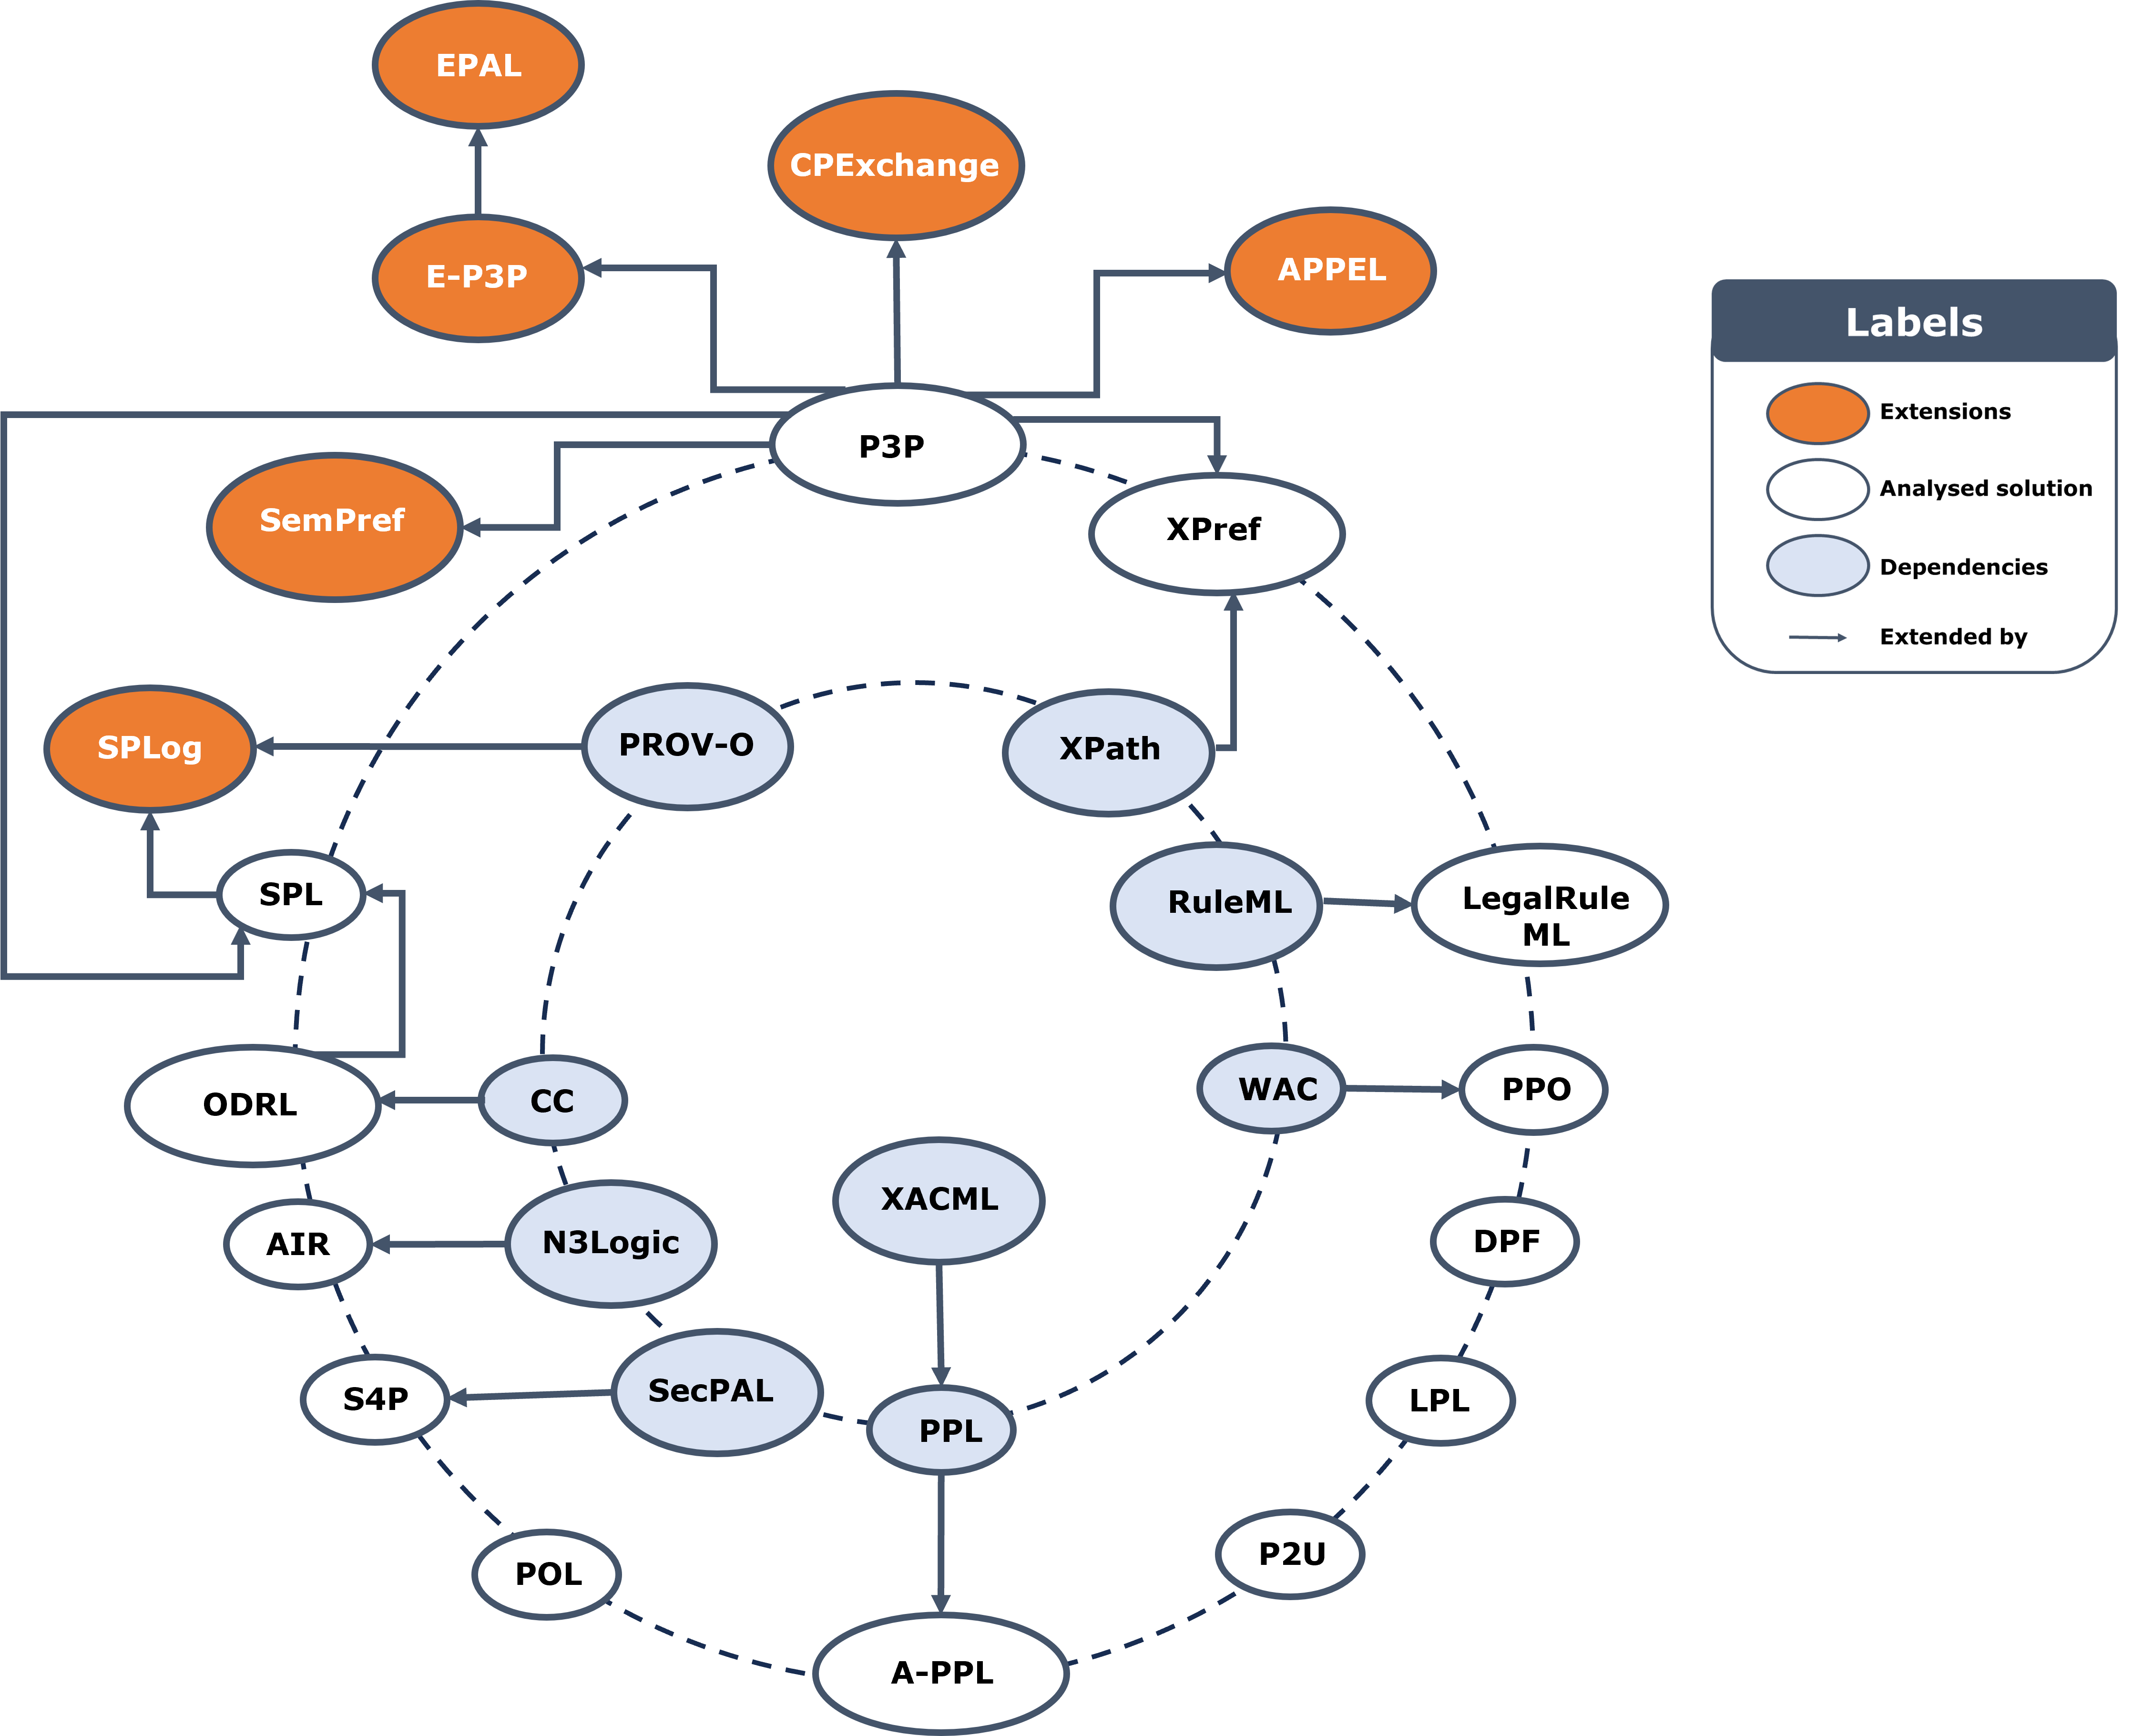
\includegraphics[width=\textwidth]{figures/chapter-2/languages.png}
    \caption{Privacy-related policy languages dependency chart.}
    \label{fig:lang-dependency-graph}
\end{figure}

Moreover, the following criteria were used to analyse existing research on semantic policy languages:
\begin{enumerate}
    \item[(C1)] Ability to model deontic concepts, e.g., permissions, prohibitions, obligations.
    \item[(C2)] Ability to model GDPR concepts, such as the privacy terms in Table~\ref{tab:GDPR_privacy_terms}.
    \item[(C3)] Existence of taxonomies of terms to populate policy conditions.
    \item[(C4)] Existence of mechanisms to assist with compliance.
    \item[(C5)] Resource is maintained/continues to be actively developed.
    \item[(C6)] Existence of an open and accessible specification.
\end{enumerate}

The outcomes of this comparative analysis will be provided in Section~\ref{sec:sota_policies_analysis} and systematised in Table~\ref{tab:languagesComparison}.

\subsection{Semantic policy languages for access control}
\label{sec:sota_policies_description}

This Section's main goal is to describe existing policy languages related to privacy, delineating the structure and information offered by each language.
Additionally, their compatibility with the GDPR is assessed, focusing on their ability to describe the provisioned rights and obligations.
Moreover, Table~\ref{tab:resources-policy-languages} provides an overview of these languages and collects information about the creators of the resources, their versions, the date of publication, and the date of the last known update.
Said languages are then analysed in chronological order regarding the date of publication and a dependency graph is presented in Figure~\ref{fig:lang-dependency-graph}.

To complement the description of the languages presented in this Section, additional documentation and resources were published on a Web page\footnote{Available at \url{https://w3id.org/people/besteves/phd/sota/languages}. Its public repository can be consulted at \url{https://w3id.org/people/besteves/phd/sota/repo} for further improvement when new solutions appear.}, including diagrams and code examples.

\subsubsection{P3P}
\label{sec:p3p}

\cite{cranor_platform_2002} introduced the Platform for Privacy Preferences (P3P) language as a standard for Web services to disclose their privacy practices in a machine-readable format.
This facilitated user agents in easily interpreting these practices and notifying users about decisions based on them. 
However, despite enabling users to be informed about the privacy policies of Web pages, these mechanisms do not ensure that the pages are actively adhering to these policies, as P3P lacks enforcement capabilities.
Therefore, the P3P vocabulary was designed not to comply with a specific regulation but rather to specify the practices of single Web pages.

The primary contributions of the P3P specification include a data schema for outlining the data intended to be collected by the Web page, a standardised set of purposes, data categories, and recipients, and an XML standard for defining privacy policies.
P3P policies consist of both general assertions and specific statements, the latter being related only to certain types of data.
General assertions encompass the legal entity applying the policy and informational elements related to access, disputes, and remedies.
The access element indicates whether the Web page allows access to the data it gathers and the disputes element outlines a process for resolving privacy-related disputes, while the remedy element details potential solutions in the event of a policy breach.
Additionally, each P3P statement consists of a distinct `data group' containing one or more data elements, along with purpose, recipient types, and retention elements.
In this context, P3P outlines a range of purposes relevant to Web-based data processing operations, such as facilitating and supporting the initial activity for which the data was supplied, conducting research and development, or performing data analysis.
%The purpose element is required to include at least one specification of purpose.
The recipient type element can be used to specify who will benefit from the collected data, while the retention element must accurately reflect the policy regarding how long the data will be kept.
Listing~\ref{list:p3p_example} displays a P3P policy that underscores the aforementioned P3P elements.
CatalogExample gathers essential details concerning its users' computer systems, as well as data regarding the pages they visit.
This information serves system administration and research and development purposes and is exclusively utilised by the company and retained for a duration deemed suitable for the specified purposes.

\begin{listing}
\caption[P3P privacy policy.]{P3P policy extracted from Example 3.1 of the P3P specification~\citep{cranor_platform_2002}, which specifies the privacy policy of CatalogExample.}
\label{list:p3p_example}
\begin{minted}{turtle}
<http://example.com/#forBrowsers> a p3p:Policy ;
    p3p:disclosure <http://example.com/PrivacyPractice.html> ;
    p3p:entity [
        p3p:business.name [ rdf:value "CatalogExample" ] ;
        p3p:business.contact-info.postal.street [
            rdf:value "4000 Lincoln Ave." ] ;
        p3p:business.contact-info.postal.city [
            rdf:value "Birmingham" ] ;
        p3p:business.contact-info.postal.stateprov [ rdf:value "MI" ] ;
        p3p:business.contact-info.postal.country [ rdf:value "USA" ] ;
        p3p:contact.online.email [ rdf:value "catalog@example.com" ] ;
        p3p:contact.telephonenum.intcode [ rdf:value "1" ] ;
        p3p:contact.telephonenum.loccode [ rdf:value "248" ] ;
        p3p:contact.telephonnum.number [ rdf:value "3926753" ] ] ;
    p3p:access p3p:AccessClass-nonident ;
    p3p:statement [
        p3p:purposeAlways p3p:Purpose-admin, p3p:Purpose-develop ;
        p3p:recipientAlways p3p:Recipient-ours ;
        p3p:retention p3p:Retention-stated-purpose ;
        p3p:data [
            rdf:predicate p3p:dynamic.clickstream, p3p:dynamic.http ] ] .
\end{minted}
\end{listing}

P3P was initially developed to articulate policies of Web services, prompting the design of APPEL as an extension to empower users in expressing their preferences~\citep{cranor_p3p_2002}.
Consequently, the utilisation of both languages becomes imperative to align user privacy preferences with service privacy policies.
Furthermore, \cite{bohrer_customer_2000} introduced the CPExchange language, an XML specification facilitating the transfer of customer data across enterprise services, incorporating P3P privacy policies relevant to the exchanged data.
Likewise, EPAL~\citep{ashley_enterprise_2003}, developed by IBM Research\footnote{\url{http://www.research.ibm.com/} (accessed on 16/July/2023)} along with its precursor E-P3P~\citep{ashley_e-p3p_2002}, leveraged P3P statements to align enterprise privacy policies with user preferences.
\cite{li_semantics-base_2006} introduces a declarative data-centric semantic model alongside a succinct syntax for P3P policies, facilitating the representation of the relationship between various P3P elements.
The primary aim of this language is to articulate policies in a manner that can be uniformly interpreted and represented across diverse user agents.
Extending this semantic foundation, the authors put forward SemPref, a preference language that considers the significance of the privacy policy rather than its syntactic form.

The P3P 1.0 Specification achieved W3C Recommendation status on April 16, 2002.
Nonetheless, its adoption was restricted as it requires acceptance from both Web services and users.
Furthermore, there has been no protocol established for these P3P policies to accurately reflect the privacy practices of Web pages.
While this specification did attain W3C recommendation status, its failure to gain widespread adoption rendered it obsolete by 2018.
Nonetheless, the significance of P3P remains considerable, as its inception and utilisation marked a pioneering endeavour in the realm of machine-readable privacy languages. 
Consequently, the primary lessons derived from this language pertain to the necessity of establishing a formal semantics capable of delineating both data subject and controller policies, which accurately reflect their data preferences and practices, and the need for tools that effectively enforce the outlined policies.

\subsubsection{ODRL}
\label{sec:odrl}

The ODRL Vocabulary \& Expression 2.2~\citep{iannella_odrl_2018} gained W3C Recommendation status in February 2018, developed by the Permissions \& Obligations Expression Working Group, with its initial version launched back in 2001.
Its primary objective was to establish a language capable of translating natural language policies into machine-readable formats, specifying details regarding permissions, prohibitions, and obligations pertaining to an asset.
This vocabulary stems from the consolidation of previous efforts undertaken by the ODRL CG, encompassing the ODRL V2.1 Common Vocabulary, the ODRL V2.1 XML Encoding, the ODRL V2.1 Ontology, and the ODRL V2.1 JSON Encoding.
Ongoing maintenance of the ODRL's standards and specifications are supported by the ODRL CG.

ODRL includes two vocabularies for the description of policies: the ODRL Core Vocabulary and the ODRL Common Vocabulary.
The primary class within ODRL's Core Vocabulary is the `policy' concept, facilitating the identification of a specific policy through its unique identifier.
Within each policy, there may exist multiple rules -- an abstract class that outlines the shared characteristics of permissions, prohibitions, and duties.
These rule types serve to declare whether a particular action, e.g., over as asset, is permitted, prohibited, or obligatory.
Additionally, permissions might also be linked with duties that must be fulfilled for said permissions to be active.
Furthermore, rules undergo further refinement through the usage of constraints, which specify the circumstances under which the rule applies, e.g., a particular permission remains valid until the conclusion of 2024.
The ODRL Vocabulary also outlines a collection of 49 actions, nine of which are imported the Creative Commons (CC) vocabulary.
The entities, or parties, involved (which can encompass a group of individuals, an organisation, or an agent) are responsible for enforcing the rules and may assume various roles contingent upon their relationship with the asset, e.g., the entity issuing the rule adopts the assigner role, whereas the recipient of the rule assumes the assignee role.
An asset, on the other hand, refers to an identifiable resource, such as data, software, services, or a combination thereof, that is subject to a rule.
The ODRL Common Vocabulary further delineates subclasses of policies, roles played by the involved parties, taxonomies of use and transfer actions for rules, and a variety of constraint operands, such as temporal, spatial, or sector-specific.
Of particular significance concerning the GDPR is the privacy policy subclass regarding assets containing personal data. 
Consequently, privacy policies implementing the ODRL language must specify to the involved parties the manner in which data is utilised, as well as with whom and for what purpose.
Listing~\ref{list:odrl_example} provides an implementation of an ODRL privacy policy that underscores the aforementioned elements, including a duty for the assignee to be allowed to use the data and a consequence in case they do not.

\begin{listing}
\caption[ODRL privacy policy.]{ODRL \texttt{Privacy} policy.}
\label{list:odrl_example}
\begin{minted}{turtle}
<http://example.com/privacy-policy> a odrl:Privacy ;
    odrl:uid <http://example.com/privacy-policy> ;
    odrl:permission [
        odrl:target <http://example.com/beatriz/contacts> ;
        odrl:assignee <http://example.com/beatriz> ;
        odrl:assigner <http://example.com/company-a> ;
        odrl:action odrl:use ;
        odrl:duty [
            odrl:action odrl:obtainConsent ;
            odrl:consentingParty <http://example.com/beatriz> ;
            odrl:consequence [
                odrl:assigner <http://example.com/company-a> ;
                odrl:action odrl:delete ] ] ] . 
\end{minted}
\end{listing}

ODRL's representational capabilities exhibit some limitations, as highlighted by~\cite{kebede_critical_2020}, particularly regarding the portrayal of delegation, the various semantics utilised for expressing duties, and the management of conflicts.
Nevertheless, efforts such as those described by~\cite{fornara_operational_2018, fornara_using_2019} are underway to formalise the semantics of ODRL policies.

ODRL was applied in various contexts, including its usage by working groups within the Open Mobile Alliance SpecWorks\footnote{\url{https://www.omaspecworks.org/} (accessed on 18/July/2023)} and by the IPTC Rights Expressions WG for the RightsML Standard\footnote{\url{https://www.iptc.org/std/RightsML/2.0/RightsML_2.0-specification.html} (accessed on 18/July/2023)}.

\subsubsection{XPref}
\label{sec:xpref}

\cite{agrawal_xpref_2005} introduced XPref as an alternative to APPEL, which only permits the definition of P3P policies that are not allowed by the user.
XPref utilises XPath (XML Path Language) 1.0 and 2.0 expressions to replace APPEL rules, enhancing the precision and reducing errors in policy formulation.
Both XPath 1.0, as described by~\cite{clark_xml_1999}, and XPath 2.0, as detailed by~\cite{berglund_xml_2010}, attained W3C Recommendation status on November 16th, 1999, and December 14th, 2010, respectively.
It should be noted that these specifications are no longer subject to further maintenance since subsequent versions have been developed.
In this context, the primary objective of XPath is to offer a method for traversing the hierarchical elements within an XML document.
In pursuit of this objective, XPath views an XML document as a tree structure of nodes
When an XPath expression is applied to the document, it determines an ordered sequence of nodes, resulting in a concise path representation.
This path consists of expressions that yield various types of nodes, including root, element, text, attribute, namespace, processing instruction, or comment nodes.

XPref was crafted to ensure that its rules not only recognise combinations of P3P elements that render a policy unacceptable based on user preferences, but also confirm that the presented elements are defined as acceptable.
It achieves these objectives while preserving the syntax and semantics of APPEL, along with its core classes.
However, the contents of the rules are substituted with XPath expressions, given that P3P policies are XML documents and can thus be readily compared with XPath-based rules.
These expressions are defined by appending a `condition' attribute to the rule, which activates the rule when the XPath expression yields a non-empty result.
%Consequently, utilising the `behavior' attribute in XPref rules allows for preferences to be set to either permit or restrict services based on the P3P policy elements they contain, such as purposes and recipients, specified in the "condition" attribute.

\subsubsection{AIR}
\label{sec:air}

In 2010, \citeauthor{hitzler_analyzing_2010} developed Accountability in RDF (AIR) -- a declarative language enabling the assertion of facts and the inclusion of rules.
AIR is built on N3Logic~\citep{berners-lee_n3logic_2008}, which supports rule nesting, rule reuse, and automated explanations of actions carried out by the AIR reasoner. 
These explanations can be customised and, given that they may contain sensitive data like Personally Identifiable Information (PII), can be employed to ensure privacy.
For example, they can be utilised to conceal actions executed under specific rules.

N3Logic extends the RDF data model with the aim of expressing logic rules on the Web, thereby promoting the use of a unified language for both data representation and logical inference.
Thus, AIR leverages N3Logic's inherent capabilities, including built-in functions, nested graphs, and contextualised reasoning.
This enables AIR rules to incorporate the usage of graphs as literal values, and built-in functions or operators defined as RDF properties.

Each AIR rule is assigned a unique IRI, ensuring its seamless integration with the linked data cloud and facilitating its reuse.
These rules adhere to the following structure: \texttt{air:if} \texttt{condition}; \texttt{air:then} \texttt{then-actions}; \texttt{air:else} \texttt{else-actions}.
The action instances can include annotations using the \texttt{air:description} property.
These annotations are subsequently integrated by the AIR reasoner into its justifications and can serve to conceal PII found within the rules.
Additionally, the format of the rules graph permits the nesting of rules within the same rule set.
This feature offers a means to segment the conditions outlined by the rule, allowing only a portion of them to be revealed in the justifications.

\subsubsection{S4P}
\label{sec:s4p}

S4P (SecPAL for Privacy), designed by \cite{becker_framework_2009, becker_s4p_2010}, constitutes a language framework designed for articulating users' privacy preferences and the data handling practices of Web services. Originating from Microsoft Research\footnote{\url{https://www.microsoft.com/en-us/research/} (accessed on 16 March 2024)}, this language serves as an extension of the company's earlier endeavor, SecPAL, aimed at delineating PII management.

SecPAL \citep{becker_design_2007} is a flexible, decentralised authorisation language, crafted for articulating policies and enhancing their expressiveness to define delegation conditions, domain-specific constraints, and negation.
An authorisation policy comprises a set of assertions, each associated with an issuer responsible for vouching for the assertion, along with a collection of conditional facts and constraints pertaining to temporal or spatial aspects.
Subsequently, when an access request is made, it undergoes a transformation into a series of queries.
These queries are then matched against the clauses that represent the system's policies, ultimately leading to a decision on data access conditions.
S4P extends SecPAL by treating granted rights and required obligations as assertions and queries.
Based on these, a satisfaction checking algorithm is formulated to evaluate the disclosure of PII between users and data-collecting services.
As a result, services should articulate their data-handling practices in the form of SecPAL queries.
Conversely, users specify their preferences as SecPAL assertions, precisely delineating what services are authorised to do and what duties they have regarding r=the usage of said PII.
% The satisfaction algorithm evaluates whether the data collection practices of the services align with the behaviors permitted by the users and whether the obligations specified in the users' preferences are adhered to by the services' policies.
If the algorithm yields a positive result, indicating that the service's policies complies with the user's preferences, the service can proceed with its data handling activities.
Additionally, S4P establishes a data disclosure protocol to ensure that users' preferences are respected when their data is shared with third party recipients.
% This protocol permits the disclosure of the user's PII only if the service's policies satisfy the user's preferences and if the policies of the third parties are in harmony with the user's preferences.

In addition to possessing an XML schema for implementation purposes, S4P features a human-readable and unambiguous syntax, enabling its utilisation in various applications. 
Listing~\ref{list:s4p_example} illustrates the S4P syntax in a scenario where Alice, the user, delineates her privacy preferences concerning the collection of her email address. 
Specifically, Alice permits eBooking services to utilise her email address for sending confirmations, newsletters, and for statistical purposes.
Additionally, Alice authorises the booking services to share her email address with trusted partners exclusively to engage with registered services that commit to deleting her email address within a month.

\begin{listing}
\caption[S4P instantiation.]{S4P example, extracted from \cite{becker_framework_2009}, which specifies Alice's privacy preferences concerning the collection of her email address by eBooking services.}
\label{list:s4p_example}
\begin{minted}[escapeinside=||]{python}
Alice says x may use Email for p if
    x is a eBookingService,
    where p |$\in$| {Confirmation, Newsletter, Stats}
Alice says x may send Email to y if
    x is a eBookingService,
    y is a TrustedPartner
Alice says x can say y is a TrustedPartner if
    x is a eBookingService
Alice says |$\langle$|Service|$\rangle$| is a RegisteredService|$?$| |$\wedge$|
    |$\exists$|t (|$\langle$|Service|$\rangle$| says |$\langle$|Service|$\rangle$| will delete Email within t|$?$| |$\wedge$| t |$\leq$| 30 days|$?$|)
\end{minted}
\end{listing}

\subsubsection{POL}
\label{sec:pol}

The Privacy Option Language (POL) was formulated by~\cite{berthold_privacy_2013} to establish privacy contracts between data controllers and data subjects, drawing on the principles of financial option contracts and corresponding data disclosure agreements.
Its architecture enforces the `data minimisation' principle by converting privacy contracts into a standard format.
This standardised format ensures that variations in contract compositions are normalised, thus providing a consistent semantic structure across contracts.

Within POL, every privacy contract is dedicated to delineating the responsibilities and entitlements concerning data disclosure.
Given its origins in the financial sphere, contract constructions in POL primarily revolve around obligations, except when a straightforward formulation of such rule types is impractical.
To specify these formulations, POL relies on various modules that are also open to extension.
The language delineates key components, including the \textbf{syntax} module, alongside modules addressing \textbf{personal data}, \textbf{purpose}, \textbf{observable} values, and \textbf{time}.
Additionally, it includes semantics modules focusing on \textbf{management} and enhancing \textbf{human readability}.
The syntax module comprises language primitives essential for defining POL contracts in their standard format.
These contracts can then integrate with data modules through various data support structures, ranging from basic attribute-value pairs, e.g., \textit{(eye colour, brown)}, to intricate tree-like data structures.
More specifically, the observable module defines comparison and Boolean operators, which are accessible within the contract execution environment, facilitating evaluations related to e.g. data retention periods.
The time module can be used to formalise different time restrictions, e.g. event-driven, discrete, or continuous time.
Furthermore, semantic modules are utilised for managing changes in observable variables, e.g., when time elapses, and for translating POL contracts into natural language.
Listing~\ref{list:pol_example} showcases the semantics of POL through a list of contracts examples:
(1) Contract $c_{company}$ delineates the immediate usage of personal data $a_1$ for purpose $p_1$;
(2) $c_{user}$ represents the negation of $c_{companyA}$ and pertains to the user disclosing the data;
(3) $c_A$ signifies a contract wherein a company holds the right to utilise data $a_A$ for purpose $p_A$ at time $t_A$ or can opt not to use it at all (represented by the $zero$ variable in the contract instantiation); and
(4) $c_B$ denotes a scenario where a company may or may not utilise data $a_B$ for purpose $p_B$ until time $t_B$ and is obligated to delete it after the deadline $t_B$.

\begin{listing}[ht]
\caption[POL contracts.]{POL contracts extracted from~\cite{berthold_towards_2011}.}
\label{list:pol_example}
\begin{minted}[escapeinside=||]{text}
(1) |$c_{company}$| = data |$a_1$| |$p_1$|
(2) |$c_{user}$| = give |$c_{company}$|
(3) |$c_A$| = when (at |$t_A$|) (data |$a_A$| |$p_A$| |`or'| zero)
(4) |$c_B$| = until (at |$t_B$|) (data |$a_B$| |$p_B$| |`or'| zero) 
\end{minted}
\end{listing}

The development of this language took place within the PETWeb II project, primarily aimed at tackling societal inquiries within the electronic identifiers domain.
The online documentation offers various application scenarios illustrating POL's utilisation.

\subsubsection{PPO}
\label{sec:ppo}

The Privacy Preference Ontology (PPO)~\citep{sacco_privacy_2011} proposes a framework for expressing users' privacy preferences regarding the restriction or allowance of access to particular RDF statements within a document.
This ontology expands upon WAC to determine users' data access rights, which is limited to specifying who can access an entire RDF document, by allowing finely-grained mechanisms for governing users' access to specific data within RDF resources.

PPO's capabilities for imposing access restrictions extend to individual statements, statement groups, and resources, which can be specific subjects or objects within RDF triples. 
Additionally, it is essential to specify the type of restriction, as users may be granted either read, write, or both access modes to the data.
By utilising the designated \textbf{hasCondition} property, specific conditions can be established to delineate privacy preferences concerning particular resources, instances of specific classes or properties, or even specific property values.
%Furthermore, it's imperative to define the access criteria to ensure that users fulfill the necessary requirements to access certain resources.
These conditions can then be checked against a SPARQL ASK query containing all the attributes and properties that users must satisfy to allow or deny access to data.

The authors also created a dedicated privacy preference manager~\citep{sacco_privacy_2011b} based on PPO.
The objective was to empower users to articulate their individual privacy preferences and manage data access based on profile attributes such as relationships, interests, or other shared characteristics.
% This ontology has the versatility to encompass social data modeled in RDF or facilitated via RDF wrappers, which can be integrated into various web pages using their Application Programming Interface (API).

\subsubsection{LegalRuleML}
\label{sec:legalruleml}

LegalRuleML, a rule language tailored to the legal domain, is developed and maintained by the OASIS\footnote{OASIS is a non-profit organisation that focuses on open standards for cloud, security and other domains, \url{https://www.oasis-open.org/} (accessed on 18/July/2023).} LegalRuleML Technical Committee and it attained OASIS Standard status in August 2021~\citep{palmirani_legalruleml_2021}.
This XML-schema specification builds upon and extends RuleML~\citep{boley_specification_2017} and incorporates formal features to represent and facilitate reasoning over legal norms, guidelines, and policies.
Key attributes of LegalRuleML include the utilisation of multiple semantic annotations for various legal interpretations, deontic operators, temporal rule management and tracking, and a mapping to RDF.

Hence, the fundamental components of a LegalRuleML document encompass \textbf{metadata}, \textbf{context}, and \textbf{statements}. 
The metadata segment comprises details concerning the \textbf{legal source} of the norms, ensuring their linkage with the corresponding legal text statements.
Additionally, it includes information about the \textbf{actors} and their \textbf{roles} in relation to the established rules, the \textbf{jurisdiction}, the \textbf{authorities} responsible for rule creation, endorsement, and enforcement, as well as temporal parameters defining rule validity.
The context element facilitates the expression of varying interpretations of rule sources, which may evolve over time or differ across jurisdictions.
It also facilitates the representation of the \textbf{association} element, establishing connections between legal sources and rules.
The statements segment involves the formalisation of norms, encompassing constitutive and prescriptive statements, as well as override and violation-reparation statements.
Constitutive rules encapsulate definitions outlined in legal documents, whereas prescriptive rules encode deontic specifications.
Override statements serve to address conflicting rules, while violation and reparation statements formalise penalties for breaches of norms.

Specifically, \cite{palmirani_modelling_2018} introduced a framework that leverages LegalRuleML, Akoma Ntoso, and the PrOnto ontology (outlined in Section~\ref{sec:pronto}) to model rules and verify compliance with GDPR's \textit{`Conditions applicable to child's consent in relation to information society services'}, described in Article 8~\citeyearpar{noauthor_regulation_2016}.

\subsubsection{A-PPL}
\label{sec:appl}

The Accountable Policy Language (A-PPL), developed by~\cite{azraoui_appl_2014}, originates from the A4Cloud\footnote{\url{http://www.a4cloud.eu/} (accessed on 19/July/2023)} project, aimed at incorporating accountability requirements into the expression of privacy policies.
To achieve this aim, A-PPL extends PPL (PrimeLife Policy Language) by integrating considerations for notification protocols, data storage and retention practices, and auditability guidelines.
PPL by~\cite{ardagna_primelife_2009} is an extensible, XACML-based \citeyearpar{parducci_extensible_2013} privacy policy language established in the context of the PrimeLife\footnote{\url{http://primelife.ercim.eu/} (accessed on 19/July/2023)} project -- XACML is an OASIS standard for access control policies that has been previously tested to deal with GDPR requirements related to consent~\citep{fatema_compliance_2017} and privacy by design~\citep{piras_defend_2019}.
The main concepts within PPL for articulating obligations consist of \textbf{triggers} and \textbf{actions}.
Triggers denote events that can undergo filtering based on specific conditions and are linked to an obligation.
These triggers are responsible for initiating actions by the data controller, which are executed in accordance with the data subject's permissions.
However, neither PPL nor XACML encompass concepts that address needs such as representing information concerning data storage and retention restrictions or incorporating auditability conditions to align with personal data protection regulations.

A-PPL incorporated a role attribute identifier and introduced the role of data protection authority to those already present in PPL, namely the data subject, data controller, and data processor.
Additionally, two new triggers for permitting or denying access to personal data were incorporated.
Duration and location attributes pertaining to specific processing activities are utilised to enforce data retention and storage rules.
Furthermore, A-PPL extends the PPL notification system by specifying the recipient and notification type to be dispatched concerning a particular action.
To facilitate auditing, A-PPL introduced a trigger to oversee the data controller's activities and gather evidence of data-related occurrences, which are logged along with parameters such as the activity's purpose, timestamp, or the executed processing operation.
Listing~\ref{list:appl_example} showcases an instance of an A-PPL obligation to inform a data subject in the event of a personal data breach -- the $ActionNotify$ element offers a mechanism for notifying data subjects, triggered in instances of policy violations or data loss.

\begin{listing}[ht]
\caption[A-PPL policy.]{A-PPL example adapted from \cite{azraoui_appl_2014}.}
\label{list:appl_example}
\begin{minted}{xml}
<Obligation>
    <TriggersSet>
        <TriggerOnPolicyViolation/>
        <TriggerOnDataLost/>
    </TriggersSet>
    <ActionNotify>
        <Media>e-mail</Media>
        <Address>data-subject@example.com</Address>
        <Recipients>Data subject</Recipients>
        <Type>Policy Violation</Type>
    </ActionNotify>
</Obligation>
\end{minted}
\end{listing}

\subsubsection{P2U}
\label{sec:p2u}

The work presented by \cite{iyilade_p2u_2014} in Purpose-To-Use (P2U) draws inspiration from P3P to construct a policy framework facilitating the sharing of user information across various services and data consumers, grounded in the principle of purpose-driven usage.
Its primary objective is to furnish a language tailored for secondary data sharing and usage, with an emphasis on safeguarding user privacy. 
P2U is structured to encompass details regarding the purpose of data sharing, its duration, and, if desired by the user, potential selling price, while also enabling data consumers to engage in negotiations concerning pricing and retention time.

This policy framework entails the interaction among distinct entities: \textbf{users} (who own the data), \textbf{data consumers} (services requiring the data), \textbf{data providers} (services gathering and sharing the data), and \textbf{data brokers} (services overseeing consumer and provider activities, including negotiation tasks).
Thus, the principal concepts of P2U are \textbf{policies}, \textbf{purposes}, \textbf{retention} restrictions, \textbf{data groups}, and their corresponding \textbf{data} elements, and the previously mentioned entities.
Policies serve as the foundational component of P2U, with each requiring an associated provider, user, and at least one designated purpose of use. 
In addition, every policy must be assigned a name and may optionally include an attribute indicating the path to a human-readable policy, as well as the name and identifier of the corresponding data provider and user. 
Within a P2U policy, multiple purposes for data sharing can be specified, along with details on retention duration, authorised recipients, and the pertinent data involved. 
Moreover, the data consumer element includes a \textbf{name} property which can be designated as `public' to allow data sharing with any third-party service. 
The duration of each purpose's retention period should be defined in days, and an optional \textbf{negotiable} property, which defaults to false, can be specified (this term can also be applied to the data group element).
The data group component comprises one or more data elements, each capable of being assigned an expiry date, which takes precedence over the retention period of the period, and the option to specify an initial price for the data, should the user opt to sell it.
Listing~\ref{list:p2u_example} illustrates an instance of a secondary data sharing P2U policy -- the data provider ``FoodIntakeApp'' wants to share Jerry's data with the data consumer ``MyShopApp'' for the purpose of shopping recommendations, allowing the consumer to retain the data for a period of 180 days and to negotiate terms with the provider.

\begin{listing}
\caption[P2U policy.]{P2U example adapted from \cite{iyilade_p2u_2014}.}
\label{list:p2u_example}
\begin{minted}{xml}
<POLICY discuri=http://mydatawebsite.com/privacy.html name="ShoppingPolicy">
    <PROVIDER name="FoodIntakeApp" provid="p6528m2" />
    <USER name="Jerry" userid="u1030050503050" />
    <PURPOSE name="Shopping Recommendations" puid="102">
        <CONSUMER name="MyShopApp" consid="c10023" />
        <RETENTION period="180" />
        <DATA-GROUP groupid="g090353" negotiable="TRUE">
            <DATA ref="#dailyfoodintake.food" sell="FALSE" />
            <DATA ref="#dailyfoodintake.quantity" sell="FALSE" />
            <DATA ref="#dailyfoodintake.hungerscale" sell="FALSE" />
        </DATA-GROUP>
    </PURPOSE>
</POLICY>
\end{minted}
\end{listing}

Another publication by the same authors~\citep{hutchison_framework_2013} outlines a scenario where a user permits data sharing among multiple mobile applications.
However, this implementation does not mandate data consumers to adhere to user-defined policies nor does it delineate any particular handling protocols for sensitive data.


\subsubsection{SPECIAL}
\label{sec:special}

The EU H2020 Scalable Policy-awarE linked data arChitecture For prIvacy, trAnsparency and compLiance (SPECIAL) project endeavoured to create technology that aids in navigating the contemporary tension between privacy and Big Data-based technologies.
As such, it aimed to furnish tools for data subjects, controllers, and processors, streamlining the management and transparent utilisation of such data.
As a result of this project, two vocabularies were developed: the SPL (SPECIAL Usage Policy Language) and the SPLog (SPECIAL Policy Log) vocabularies~\citep{gangemi_scalable_2018}.

A SPL usage policy delineates a collection of permissible actions aligned with the consent of the data subject.
To formalise these actions in accordance with GDPR requirements, SPL outlines five fundamental concepts: the \textbf{data} subjected to processing, the intended \textbf{purpose} of such processing, detailed information of the \textbf{processing} operation, information regarding \textbf{storage}, and the designated \textbf{recipients} of the processing outcomes. 
The data storage term encompasses the specification of two attributes: the storage location and duration.
Therefore, in mathematical terms, the usage policy is represented as a tuple consisting of five elements, each representing an instantiation of the five core classes, thereby defining a permitted activity.
Moreover, a composed usage policy can be formulated by joining a set of authorised processing activities.
The vocabularies crafted to delineate each concept within the SPL construct draw upon established privacy-related ontologies.
For instance, terms related to processing operations\footnote{\url{https://specialprivacy.ercim.eu/vocabs/processing\#} (accessed on 20/July/2023)} are derived from previous ontologies such as ODRL, while data categories\footnote{\url{https://specialprivacy.ercim.eu/vocabs/data\#} (accessed on 20/July/2023)}, recipients\footnote{\url{https://specialprivacy.ercim.eu/vocabs/recipients\#} (accessed on 20/July/2023)}, purposes\footnote{\url{https://specialprivacy.ercim.eu/vocabs/purposes\#} (accessed on 20/July/2023)}, storage duration\footnote{\url{https://specialprivacy.ercim.eu/vocabs/duration\#} (accessed on 20/July/2023)}, and location\footnote{\url{https://specialprivacy.ercim.eu/vocabs/locations\#} (accessed on 20/July/2023)} are derived from P3P.
These taxonomies have the potential for expansion through the introduction of additional sub-classes~\citep{bonatti_policy_2018}.
An example showcasing this extension possibility is illustrated in Listing~\ref{list:spl_example}, where the terms \texttt{HeartRate}, a sub-class of \texttt{svd:Health}, \texttt{Profiling} a sub-class of the processing term \texttt{svpr:Analyze}, and \texttt{Recommendation} as a subclass of the purpose \texttt{svpu:Marketing}, are introduced. 
In this example, data concerning heart rate and location are utilised for user profiling with the aim of generating recommendations, while the data is stored indefinitely within the servers of the data controllers situated in the EU and may be disclosed to any recipients.

\begin{listing}
\caption[SPL general usage policy.]{SPL general usage policy adapted from \cite{bonatti_special_2019}.}
\label{list:spl_example}
\begin{minted}{text}
ObjectIntersectionOf(
    ObjectSomeValueFrom( spl:hasData
        ObjectUnionOf( ex:HeartRate svd:Location ))
    ObjectSomeValueFrom( spl:hasProcessing ex:Profiling )
    ObjectSomeValueFrom( spl:hasPurpose ex:Recommendation )
    ObjectSomeValueFrom( spl:hasStorage
        ObjectIntersectionOf(
            ObjectSomeValuesFrom( spl:hasLocation
                ObjectIntersectionOf( svl:OurServers svl:EU ))
            DataSomeValuesFrom( spl:durationInDays
                DatatypeRestriction( xsd:integer
                    xsd:mininclusive "0"^^xsd:integer ))))
    ObjectSomeValueFrom( spl:hasRecipient spl:AnyRecipient ))
\end{minted}
\end{listing}

SPLog was developed to document the processing events associated with the consent actions granted by data subjects.
It leverages PROV-O~\citep{lebo_prov-o_2013} to incorporate provenance information into the log, aligning with the terminology established for the SPL vocabulary. 
The key concepts outlined by SPLog encompass the \textbf{log} itself and the corresponding \textbf{log entries}.
Each log is accompanied by metadata, including the software agent to which it pertains, while log entries provide details about individual events. 
These entries can be categorised into two types: policy entries, which are linked to consent forms and associated terms, and data events, e.g., processing or sharing activities. 
Additionally, these entries should encompass information regarding the involved data subject, event description, content, timestamps, and relevant datasets, facilitating the tracking of event provenance.
Hence, SPLog utilises the SPL vocabulary to instantiate the content of a log entry, which allows event grouping to enhance scalability~\citep{kirrane_transparency_2018}.

The SPECIAL framework found application across diverse sectors through various use cases: collaborating with \textit{Proximus}\footnote{\url{https://www.proximus.be/} (accessed on 20/July/2023)} to develop personalised tourist recommendations; partnering with \textit{Deutsche Telekom}\footnote{\url{https://www.telekom.com/en} (accessed on 20/July/2023)} to deliver traffic alert notifications; and working alongside \textit{Thomson Reuters Limited}\footnote{\url{https://www.thomsonreuters.com} (accessed on 20/July/2023)} to address anti-money laundering requirements.

\subsubsection{DPF}
\label{sec:dpf}

The Declarative Policy Framework (DPF), as documented by \cite{martiny_protecting_2018} and \cite{martiny_partial_2020}, was developed as part of the DARPA Brandeis program\footnote{\url{https://www.darpa.mil/program/brandeis} (accessed on 20/July/2023)}.
Its primary objective is to furnish a privacy policy framework grounded in ontology engineering principles and a formal theory of shareability.
DPF's policy engine utilises the ontology to delineate policy instantiations, which subsequently inform the generation of user interfaces. 
These interfaces are designed to empower non-technical users to generate, validate, and manage privacy policies, alleviating them from the intricacies of technical policy language formalisms.
Furthermore, DPF's engine is adaptable for integration into systems that support data request management and other Privacy Enhancing Technologies (PETs).

Thus, DPF employs a predefined ontology as a common data model to articulate a specific domain, facilitating the formulation of both permissive and prohibitive privacy policies. 
Each policy rule encompasses either an allowance or denial statement, necessitating an identifier, a description, an authority, designated data requesters, and the pertinent data affected by the policy, along with the timeframe of its effectiveness. 
In instances of permissive statements, there is the option to outline a set of constraints that dictate the circumstances under which data may be shared. 
The policy authority is responsible for assessing whether a given data request aligns with the established policies.
Consequently, each data request must include not only the requested data but also the consulted policy authority tasked with granting or denying access, as well as the request timestamp.
Subsequently, the request travels through the policy engine pipeline, and upon encountering a matching rule, the engine furnishes the decision along with the identifier and description of the corresponding rule.
If the request is authorised, the engine also provides the valid conditions under which it is permissible. 
Given that a single request may trigger multiple policy rules, the engine must effectively manage conflicting decisions.
To address this, DPF incorporates baseline policies, and exceptions are established to delineate policy rules with higher priority concerning the shared data. 
Through this mechanism, this privacy framework is capable of overriding decisions based on specific constraints.

The ontologies are specified in OWL and can be converted to Flora\footnote{\url{http://flora.sourceforge.net/} (accessed on 20/July/2023)}, an object-oriented reasoning system. 
To demonstrate this framework, the authors offer a pandemic use case wherein national and community policy authorities establish data-sharing policies concerning their residents' health statuses to monitor disease outbreaks. 
In Listing~\ref{list:dpf_example}, an example DPF policy rule is provided based on this scenario.
Any national policy authority, $?pa$, permits nations to share information regarding their residents' disease states, $?reqData$, with response coordinators, $?requester$, at a specified time, $?time$, subject to certain constraints, $?constr$. 
The $?polData$ query delineates the relationship between nations and the medical statuses of their residents, constrained by $?constr$, which is attached to the $?Resident$ variable.
Within this constraint, the birthday of the resident is considered to exclude residents younger than thirteen from the requested data.

\begin{listing}[ht]
\caption[DPF policy.]{DPF constrained policy rule adapted from \cite{martiny_protecting_2018}.}
\label{list:dpf_example}
\begin{minted}[escapeinside=||]{text}
@!{NationsAllowConstrainedDiseaseStatesToRCs}
?pa [allow_sa(?requester, ?reqData, ?time, ?constr, ?id, ?descr, 0)] :-
    ?id = "NationsAllowConstrainedDiseaseStatesToRCs"^^\string,
    ?descr = "Nations share disease states w Response Coordinators"^^\string,
    ?pa : NationPolicyAuthority,
    ?requester : ResponseCoordinator,
    ?polData = |$\textdollar$|{ ?pa [nation -> ?Nation],
        ?Nation : Nation [community -> ?Community, name -> ?NationName],
        ?Community : Community [resident -> ?Resident],
        ?Resident : Person [medicalInformation -> ?MedInfo],
        ?MedInfo : DiseaseStatus [state -> ?MedState],
        ?Resident [constraints -> ?constr] },
    ?thirteenYears is 13*365*24*60*60, 
    ?time [subtractTime(?thirteenYears) -> ?latestTime],
    ?constr = [|$\textdollar$|{ 
        ?Resident : Person [birthDate -> ?Birthdate],
        timeBefore(?Birthdate, ?latestTime) }],
    implies_sharing(?polData, ?reqData, ?constr).
\end{minted}
\end{listing}

\subsubsection{LPL}
\label{sec:lpl}

The Layered Privacy Language (LPL), as developed by~\cite{gerl_lpl_2018}, is a privacy language designed to be comprehensible by both humans and machines.
Its primary objective is to facilitate the expression and enforcement of GDPR's requirements pertaining to data subject consent, personal data provenance, retention, and the implementation of privacy-preserving processing activities utilising advanced anonymisation techniques.
In subsequent research by~\cite{gerl_critical_2018}, efforts were directed towards enhancing LPL to comprehensively address the requirements outlined in Articles 12 to 14 of the GDPR, collectively known as the data subject's `Right to be informed'.

The policy structure of LPL is organised around purposes.
In this structure, a collection of \textbf{purposes} forms the core architecture, with each purpose being associated with a set of processed \textbf{data} types and their corresponding \textbf{recipients}.
Moreover, the purpose element can be enriched with a human-readable description and also includes properties such as \textbf{required}, which specifies whether a particular purpose needs explicit consent from the data subject, and \textbf{optOut}, indicating whether the user must actively accept or decline the purpose.
Data elements serve to identify the data group to which the processed data belongs, as well as categorise them as sensitive or explicit.
Alongside data recipients, other entities like data controllers or the data protection officer can also be designated with LPL.
Furthermore, LPL policies can include details on the retention period, data subject's rights, legal basis, and description details pertaining to automated decision-making activities.
The example LPL policy provided in Listing~\ref{list:lpl_example} illustrates how company $dr_{C1}$ operates its personal data handling activities under the LPL privacy policy $lpp_{ds_{U1}-dr_{C1}}$.
This policy governs the collection and usage of personal information from a user $ds_{U1}$ for a specific purpose $p_{U1}$.
Additionally, it allows for the optional sharing of collected data with a third-party recipient.
Should such sharing occur, a new contract must be established, with company $C1$ ($ds_{C1}$) acting as the data source and the third party $C2$ ($dr_{C2}$) as the data recipient.
The purpose of processing, denoted as $p_{U1}$, is `Marketing', involving personal data $\hat{D}_1$ such as postal code (anonymised via the `Suppression' method) and salary information, which must be deleted within 180 days following the fulfilment of the purpose.

\begin{listing}[ht]
\caption[LPL policy.]{LPL policy extracted from \cite{gerl_lpl_2018}.}
\label{list:lpl_example}
\begin{minted}[escapeinside=||]{text}
|$ds_{U1}$|=('U1','Person',|$publicKey_{U1}$|,'DataSource')
|$dr_{C1}$|=('C1','Legal Entity',|$publicKey_{C1}$|,'DataRecipient')
|$ds_{C1}$|=('C1','Legal Entity',|$publicKey_{C1}$|,'DataSource')
|$dr_{C2}$|=('C2','Legal Entity',|$publicKey_{C2}$|,'DataRecipient')
|$lpp_{ds_{U1}-dr_{C1}}$|=('1','LPP1','en','https://company.com/privacy.html',|$\emptyset$|,|$ds_{U1}$|,{|$p_{U1}$|})
|$p_{U1}$|=('Marketing','false','true','Marketing purposes, including newsletters.',{|$dr_{C1}$|,|$dr_{C2}$|},|$r_1$|,pm,|$\hat{D}_1$|)
|$r_1$|=('AfterPurpose','180 days')
|$\hat{D}_1$|={|$d_{postal}$|,|$d_{salary}$|}
|$d_{postal}$|=('postal-code',dGroup,'Number','true','Postal code of the user','QID',am1)
|$am_1$|=('Suppression',{|$ama_1$|,|$ama_2$|,|$ama_3$|,|$ama_4$|},|$\emptyset$|)
|$ama_1$|=('Suppression Replacement','*')
|$ama_2$|=('Suppression Direction','backward')
|$ama_3$|=('Minimum Level','2')
|$ama_4$|=('Maximum Level','4')
|$d_{salary}$|=('salary',dGroup,'Number','true','Monthly salary amount received by the user','Sensitive',|$\emptyset$|)
\end{minted}
\end{listing}

\cite{gerl_privacy_2019} conducted validation of this language through a real-world use-case scenario within the healthcare domain, showcasing its effectiveness and constraints concerning GDPR compliance.
Subsequent research expanded upon LPL by integrating machine-readable privacy icons~\citep{gerl_extending_2018}, aiming to evaluate their impact on the comprehension of privacy policies.
Additionally, an LPL Personal Privacy Policy User Interface was introduced~\citep{gerl_interface_2018}.
This interface primarily aims to present information pertinent to privacy policies, aiding data subjects in providing informed consent.
It includes a policy header containing a link to the human-readable policy and an overview of processing purposes using the previously mentioned privacy icons.
Furthermore, a purpose section outlines all purposes outlined in the privacy policy, along with details regarding data controllers, recipients, retention periods, and anonymisation methods.

\subsection{Comparative analysis}
\label{sec:sota_policies_analysis}

Using Table~\ref{tab:languagesComparison}, it is possible to assess and compare the policy languages outlined in this Section, regarding their effectiveness in aiding the representation of GDPR rights and obligations. 
The languages in the Table are arranged firstly by the number of supported criteria in descending order, followed by alphabetical sorting if needed, to enhance clarity and readability.

\begin{table}[ht]
\centering
\caption[Comparison of the analysed privacy policy languages.]{Comparison of the analysed privacy policy languages, according to the defined criteria described in Section \ref{sec:sota_policies_criteria}.}
\label{tab:languagesComparison} 
\begin{tabular}{ c||c|c|c|c|c|c}
 & C1 & C2 & C3 & C4 & C5 & C6 \\
 \hline\hline
 LegalRuleML & Yes & Partially & No & Yes & Yes & Yes \\
 \hline
 ODRL & Yes & Partially & Yes & No & Yes & Yes \\
  \hline
 SPL & No & Partially & Yes & Yes & No & Yes \\
 \hline
  A-PPL & Yes & Partially & No & Yes & No & No \\
 \hline
  DPF & Yes & Partially & No & Yes & Unknown & No \\
 \hline
  P3P & No & Partially & Yes & No & No & Yes \\
 \hline
  AIR & No & No & No & Yes & No & Yes \\
 \hline
  LPL & No & Partially & No & Yes & Unknown & No \\
  \hline
 S4P & No & Partially & No & Yes & No & No \\
 \hline
  P2U & No & Partially & No & No & No & No \\
 \hline
 POL & No & Partially & No & No & No & No \\
 \hline
  PPO & No & No & No & No & No & No \\
  \hline
 XPref & No & No & No & No & No & No \\
\end{tabular}
\end{table}

While these languages may not explicitly address the rights and obligations outlined in Section~\ref{sec:def_gdpr}, they can still encapsulate some of the information items discussed therein.
Thus, they are categorised as partially capable of representing GDPR concepts and principles (C2 criterion in Table~\ref{tab:languagesComparison}).
Most of the examined languages can partially fulfil the representational requirements of GDPR as identified in Table~\ref{tab:GDPR_privacy_terms}, with the exceptions being AIR, PPO, and XPref.
Examples illustrating how to encode specific aspects of privacy policies for each language partially capable of representing GDPR concepts are provided in Listings~\ref{list:p3p_example} to~\ref{list:lpl_example}.

Among these languages, only ODRL, SPL, and P3P offer taxonomies for populating policies.
Moreover, only LegalRuleML, ODRL, A-PPL, and DPF incorporate deontic concepts like permissions or obligations into their models.
In their documentation, LegalRuleML, SPL, A-PPL, DPF, AIR, LPL, and S4P also acknowledge the presence of reasoning mechanisms or other supportive tools, which leverage the implemented languages to aid in compliance efforts.
Some of these languages also provide access to such tools.
Nevertheless, LegalRuleML and ODRL are the only languages that are actively maintained and developed, while, among the languages examined, only LegalRuleML, ODRL, SPL, P3P, and AIR offer resources that can be readily reused on the Web.

Notably, LegalRuleML and ODRL distinguish themselves from other languages by possessing the capabilities to positively address a larger proportion of the established comparison criteria, including the ability to model deontic concepts and GDPR terms, e.g., purposes or data recipients.
Moreover, their development and extension can be supported by the community groups in charge of their maintenance, and their resources are open and accessible.
Beyond this, ODRL also supports the modelling of other constraints with particular importance in the definition of access control policies, e.g., spatial and temporal constraints, the representation of distinct types of policies, e.g., offers, requests and agreements, and has a profile mechanism to develop extensions to its core vocabulary.
As such, ODRL will be the basis upon which access policies are expressed in this Thesis.
\section{Gaps and challenges}
\label{sec:challenges}

This Section discusses the challenges of having a transparent, legally-aligned Solid ecosystem based on the literature review described in this Chapter. The following issues were identified based on the performed analysis:

\begin{enumerate} % copy from PLASMA paper
    \item [Ch1.] \textbf{Identity of Solid actors and their roles is unknown} -- Solid users are unaware of who are the entities providing and/or developing their Pods, the apps they use, WebIDs, or server infrastructure and implementation. Furthermore, most apps or services do not provide contact details or information regarding their data protection officer.
    \item [Ch2.] \textbf{No metadata about Solid infrastructure} -- Solid users do not have information on which Solid specification their Pod is running, which functionalities are installed within it or where are the servers located. Moreover, no record of this information is kept in the Pod for easy consultation by the user.\footnote{A non-exhaustive list of Pod providers is available at \url{https://solidproject.org/users/get-a-pod}, with information on the service used to host the Pods (but no information on the entities behind them) and, in some cases, the country where it is hosted (but no privacy policy for the storage service is provided).}
    \item [Ch3.] \textbf{Availability/Discovery of categories of data} -- To have granular access to data in Pods, based on their data category, Solid apps need to know if they exist and where are they stored in the Pod. Moreover, for seamless interoperability, schemas, formats or shapes for data recognised or supported by apps, services or Pods need to be recorded.
    \item [Ch4.] \textbf{Pod and app providers do not provide information on their data handling practices} -- Most providers and developers of Pod-related services do not provide human and/or machine-readable privacy notices nor do they declare what data they need to function. Such information also needs to be recorded in the Pod so that users can have a copy of the user/app request for data, e.g., in case data is used in a way that was not permitted by its data subject.
    \item [Ch5.] \textbf{Users cannot express their privacy policies} -- Solid users do not have the tools to express their privacy preferences and requirements nor to manage incoming data requests or existing decisions for the usage of data.
    \item [Ch6.] \textbf{No logging or record-keeping} -- No provenance metadata is recorded for accountability in the user Pod, e.g., users do not keep consent records, nor information regarding who has accessed their data, what they are doing with it, or changes to their data handling policies.
    \item [Ch7.] \textbf{No legal compliance checks} -- Solid does not provide its users with the tools to deal with legal requirements, such as giving/withdrawing consent or exercising rights under the GDPR, nor does it provide authorities with the auditing information to perform investigations.
\end{enumerate}